\documentclass[11pt]{article}
% =======================================================================
%   Shared style for CS 300 notes.
%   Usage: place `% =======================================================================
%   Shared style for CS 300 notes.
%   Usage: place `% =======================================================================
%   Shared style for CS 300 notes.
%   Usage: place `\input{../../notes-style.tex}` right after \documentclass
%   in each chapter's lectures.tex and notes.tex.
% =======================================================================

% ---- Layout -----------------------------------------------------------
\usepackage[margin=1in]{geometry}
\usepackage{parskip}        % space between paragraphs, no indent
\usepackage{microtype}      % subtle kerning/spacing improvements

% ---- Colors (muted palette, easy on light-sensitive eyes) -------------
\usepackage{xcolor}
\definecolor{pagebg}       {HTML}{FAF6F0}  % warm cream background
\definecolor{bodyfg}       {HTML}{3D3A36}  % warm dark gray body text
\definecolor{heading}      {HTML}{3D6A6B}  % muted teal
\definecolor{subheading}   {HTML}{5B7A9C}  % dusty blue
\definecolor{accent}       {HTML}{8A6B4A}  % warm tan
\definecolor{linkcol}      {HTML}{5B7A9C}  % same as subheading
\definecolor{mutedtext}    {HTML}{6B6560}  % secondary / caption text
\definecolor{rulecol}      {HTML}{C8BFB0}  % separator / rule

% Callout box palette
\definecolor{defnFrame}    {HTML}{9DB89B}  \definecolor{defnBack}    {HTML}{EEF2E8}
\definecolor{ideaFrame}    {HTML}{9FB4CD}  \definecolor{ideaBack}    {HTML}{E8EEF5}
\definecolor{warnFrame}    {HTML}{CFAE87}  \definecolor{warnBack}    {HTML}{F5EDDF}
\definecolor{noteFrame}    {HTML}{BFA6AE}  \definecolor{noteBack}    {HTML}{F2E8EE}
\definecolor{exFrame}      {HTML}{9FBDBD}  \definecolor{exBack}      {HTML}{E8F0F0}
\definecolor{codeBack}     {HTML}{F3EDE2}
\definecolor{codeBorder}   {HTML}{D4CBBA}
\definecolor{codeKeyword}  {HTML}{6B4F7A}
\definecolor{codeString}   {HTML}{8A6B4A}
\definecolor{codeComment}  {HTML}{8A857F}

% ---- Page background + base text color --------------------------------
\usepackage{pagecolor}
\pagecolor{pagebg}
\color{bodyfg}

% ---- Fonts ------------------------------------------------------------
\usepackage[T1]{fontenc}
\IfFileExists{libertine.sty}{%
    \usepackage{libertine}      % warm, readable serif
    \usepackage[scaled=0.95]{inconsolata}  % softer monospace
}{}

% ---- Hyperref ---------------------------------------------------------
\usepackage{hyperref}
\hypersetup{
    colorlinks=true,
    linkcolor=linkcol,
    urlcolor=linkcol,
    citecolor=linkcol,
    pdfborder={0 0 0},
}

% ---- Section styling --------------------------------------------------
\usepackage[explicit]{titlesec}
\titleformat{\section}
    {\color{heading}\Large\bfseries}
    {\color{heading}\thesection\hspace{0.6em}}{0pt}{#1}
\titleformat{\subsection}
    {\color{subheading}\large\bfseries}
    {\color{subheading}\thesubsection\hspace{0.5em}}{0pt}{#1}
\titleformat{\subsubsection}
    {\color{accent}\normalsize\bfseries}
    {\color{accent}\thesubsubsection\hspace{0.5em}}{0pt}{#1}
\titleformat{\paragraph}[runin]
    {\color{accent}\bfseries}{}{0pt}{#1.}

\titlespacing*{\section}{0pt}{1.6em}{0.6em}
\titlespacing*{\subsection}{0pt}{1.2em}{0.4em}

% ---- Enumerate / itemize spacing --------------------------------------
\usepackage{enumitem}
\setlist[itemize]{leftmargin=1.4em, itemsep=2pt, topsep=4pt}
\setlist[enumerate]{leftmargin=1.6em, itemsep=2pt, topsep=4pt}

% ---- Code listings ----------------------------------------------------
\usepackage{listings}
\lstdefinestyle{notescode}{
    backgroundcolor=\color{codeBack},
    basicstyle=\ttfamily\small\color{bodyfg},
    keywordstyle=\color{codeKeyword}\bfseries,
    stringstyle=\color{codeString},
    commentstyle=\color{codeComment}\itshape,
    frame=single,
    framesep=6pt,
    rulecolor=\color{codeBorder},
    showstringspaces=false,
    breaklines=true,
    xleftmargin=10pt,
    xrightmargin=10pt,
    aboveskip=8pt,
    belowskip=8pt,
}
\lstset{style=notescode}

% ---- Callout boxes (tcolorbox) ----------------------------------------
\usepackage[most]{tcolorbox}

\newtcolorbox{defnbox}[1][]{
    enhanced, breakable,
    colback=defnBack, colframe=defnFrame, coltitle=bodyfg,
    title={\bfseries Definition \textemdash\ #1},
    fonttitle=\bfseries,
    boxrule=0.5pt, arc=2pt, left=8pt, right=8pt, top=6pt, bottom=6pt,
    attach boxed title to top left={xshift=10pt, yshift=-6pt},
    boxed title style={colback=defnFrame, colframe=defnFrame, arc=2pt},
    before skip=8pt, after skip=8pt,
}
\newtcolorbox{ideabox}[1][]{
    enhanced, breakable,
    colback=ideaBack, colframe=ideaFrame, coltitle=bodyfg,
    title={\bfseries Key idea #1},
    boxrule=0.5pt, arc=2pt, left=8pt, right=8pt, top=6pt, bottom=6pt,
    attach boxed title to top left={xshift=10pt, yshift=-6pt},
    boxed title style={colback=ideaFrame, colframe=ideaFrame, arc=2pt},
    before skip=8pt, after skip=8pt,
}
\newtcolorbox{warnbox}[1][]{
    enhanced, breakable,
    colback=warnBack, colframe=warnFrame, coltitle=bodyfg,
    title={\bfseries Gotcha #1},
    boxrule=0.5pt, arc=2pt, left=8pt, right=8pt, top=6pt, bottom=6pt,
    attach boxed title to top left={xshift=10pt, yshift=-6pt},
    boxed title style={colback=warnFrame, colframe=warnFrame, arc=2pt},
    before skip=8pt, after skip=8pt,
}
\newtcolorbox{notebox}[1][]{
    enhanced, breakable,
    colback=noteBack, colframe=noteFrame, coltitle=bodyfg,
    title={\bfseries Aside #1},
    boxrule=0.5pt, arc=2pt, left=8pt, right=8pt, top=6pt, bottom=6pt,
    attach boxed title to top left={xshift=10pt, yshift=-6pt},
    boxed title style={colback=noteFrame, colframe=noteFrame, arc=2pt},
    before skip=8pt, after skip=8pt,
}
\newtcolorbox{examplebox}[1][]{
    enhanced, breakable,
    colback=exBack, colframe=exFrame, coltitle=bodyfg,
    title={\bfseries Example #1},
    boxrule=0.5pt, arc=2pt, left=8pt, right=8pt, top=6pt, bottom=6pt,
    attach boxed title to top left={xshift=10pt, yshift=-6pt},
    boxed title style={colback=exFrame, colframe=exFrame, arc=2pt},
    before skip=8pt, after skip=8pt,
}

% ---- TikZ graph styles (added 2026-04-25 for ch_10 augmentation) ------
% tcolorbox[most] already loads tikz; this block declares the libraries
% + shared `vertex` / `edge` styles used by ch_10's general directed-graph
% diagrams. ch_9's tree-style TikZ uses inline overrides and is
% unaffected. Simple circle nodes + arrow edges only -- no production
% styling.
\usetikzlibrary{arrows.meta, positioning, calc}
\tikzset{
    vertex/.style={circle, draw, minimum size=7mm, inner sep=0pt,
                   font=\small, thick},
    vsource/.style={vertex, fill=ideaBack},
    vdone/.style={vertex, fill=defnBack},
    edge/.style={->, >=Stealth, thick},
    uedge/.style={-, thick},
    treeedge/.style={->, >=Stealth, thick},
    backedge/.style={->, >=Stealth, thick, dashed, red!70!black},
    fwdedge/.style={->, >=Stealth, thick, blue!60!black},
    crossedge/.style={->, >=Stealth, thick, green!50!black, dotted},
    mstedge/.style={-, very thick, accent},
}

% ---- Title block ------------------------------------------------------
\usepackage{titling}
\pretitle{\begin{center}\color{heading}\LARGE\bfseries}
\posttitle{\end{center}\vskip -0.4em}
\preauthor{\begin{center}\color{mutedtext}\normalsize}
\postauthor{\end{center}}
\predate{\begin{center}\color{mutedtext}\small}
\postdate{\end{center}\vspace{0.4em}{\color{rulecol}\hrule height 0.4pt}\vspace{1.2em}}
` right after \documentclass
%   in each chapter's lectures.tex and notes.tex.
% =======================================================================

% ---- Layout -----------------------------------------------------------
\usepackage[margin=1in]{geometry}
\usepackage{parskip}        % space between paragraphs, no indent
\usepackage{microtype}      % subtle kerning/spacing improvements

% ---- Colors (muted palette, easy on light-sensitive eyes) -------------
\usepackage{xcolor}
\definecolor{pagebg}       {HTML}{FAF6F0}  % warm cream background
\definecolor{bodyfg}       {HTML}{3D3A36}  % warm dark gray body text
\definecolor{heading}      {HTML}{3D6A6B}  % muted teal
\definecolor{subheading}   {HTML}{5B7A9C}  % dusty blue
\definecolor{accent}       {HTML}{8A6B4A}  % warm tan
\definecolor{linkcol}      {HTML}{5B7A9C}  % same as subheading
\definecolor{mutedtext}    {HTML}{6B6560}  % secondary / caption text
\definecolor{rulecol}      {HTML}{C8BFB0}  % separator / rule

% Callout box palette
\definecolor{defnFrame}    {HTML}{9DB89B}  \definecolor{defnBack}    {HTML}{EEF2E8}
\definecolor{ideaFrame}    {HTML}{9FB4CD}  \definecolor{ideaBack}    {HTML}{E8EEF5}
\definecolor{warnFrame}    {HTML}{CFAE87}  \definecolor{warnBack}    {HTML}{F5EDDF}
\definecolor{noteFrame}    {HTML}{BFA6AE}  \definecolor{noteBack}    {HTML}{F2E8EE}
\definecolor{exFrame}      {HTML}{9FBDBD}  \definecolor{exBack}      {HTML}{E8F0F0}
\definecolor{codeBack}     {HTML}{F3EDE2}
\definecolor{codeBorder}   {HTML}{D4CBBA}
\definecolor{codeKeyword}  {HTML}{6B4F7A}
\definecolor{codeString}   {HTML}{8A6B4A}
\definecolor{codeComment}  {HTML}{8A857F}

% ---- Page background + base text color --------------------------------
\usepackage{pagecolor}
\pagecolor{pagebg}
\color{bodyfg}

% ---- Fonts ------------------------------------------------------------
\usepackage[T1]{fontenc}
\IfFileExists{libertine.sty}{%
    \usepackage{libertine}      % warm, readable serif
    \usepackage[scaled=0.95]{inconsolata}  % softer monospace
}{}

% ---- Hyperref ---------------------------------------------------------
\usepackage{hyperref}
\hypersetup{
    colorlinks=true,
    linkcolor=linkcol,
    urlcolor=linkcol,
    citecolor=linkcol,
    pdfborder={0 0 0},
}

% ---- Section styling --------------------------------------------------
\usepackage[explicit]{titlesec}
\titleformat{\section}
    {\color{heading}\Large\bfseries}
    {\color{heading}\thesection\hspace{0.6em}}{0pt}{#1}
\titleformat{\subsection}
    {\color{subheading}\large\bfseries}
    {\color{subheading}\thesubsection\hspace{0.5em}}{0pt}{#1}
\titleformat{\subsubsection}
    {\color{accent}\normalsize\bfseries}
    {\color{accent}\thesubsubsection\hspace{0.5em}}{0pt}{#1}
\titleformat{\paragraph}[runin]
    {\color{accent}\bfseries}{}{0pt}{#1.}

\titlespacing*{\section}{0pt}{1.6em}{0.6em}
\titlespacing*{\subsection}{0pt}{1.2em}{0.4em}

% ---- Enumerate / itemize spacing --------------------------------------
\usepackage{enumitem}
\setlist[itemize]{leftmargin=1.4em, itemsep=2pt, topsep=4pt}
\setlist[enumerate]{leftmargin=1.6em, itemsep=2pt, topsep=4pt}

% ---- Code listings ----------------------------------------------------
\usepackage{listings}
\lstdefinestyle{notescode}{
    backgroundcolor=\color{codeBack},
    basicstyle=\ttfamily\small\color{bodyfg},
    keywordstyle=\color{codeKeyword}\bfseries,
    stringstyle=\color{codeString},
    commentstyle=\color{codeComment}\itshape,
    frame=single,
    framesep=6pt,
    rulecolor=\color{codeBorder},
    showstringspaces=false,
    breaklines=true,
    xleftmargin=10pt,
    xrightmargin=10pt,
    aboveskip=8pt,
    belowskip=8pt,
}
\lstset{style=notescode}

% ---- Callout boxes (tcolorbox) ----------------------------------------
\usepackage[most]{tcolorbox}

\newtcolorbox{defnbox}[1][]{
    enhanced, breakable,
    colback=defnBack, colframe=defnFrame, coltitle=bodyfg,
    title={\bfseries Definition \textemdash\ #1},
    fonttitle=\bfseries,
    boxrule=0.5pt, arc=2pt, left=8pt, right=8pt, top=6pt, bottom=6pt,
    attach boxed title to top left={xshift=10pt, yshift=-6pt},
    boxed title style={colback=defnFrame, colframe=defnFrame, arc=2pt},
    before skip=8pt, after skip=8pt,
}
\newtcolorbox{ideabox}[1][]{
    enhanced, breakable,
    colback=ideaBack, colframe=ideaFrame, coltitle=bodyfg,
    title={\bfseries Key idea #1},
    boxrule=0.5pt, arc=2pt, left=8pt, right=8pt, top=6pt, bottom=6pt,
    attach boxed title to top left={xshift=10pt, yshift=-6pt},
    boxed title style={colback=ideaFrame, colframe=ideaFrame, arc=2pt},
    before skip=8pt, after skip=8pt,
}
\newtcolorbox{warnbox}[1][]{
    enhanced, breakable,
    colback=warnBack, colframe=warnFrame, coltitle=bodyfg,
    title={\bfseries Gotcha #1},
    boxrule=0.5pt, arc=2pt, left=8pt, right=8pt, top=6pt, bottom=6pt,
    attach boxed title to top left={xshift=10pt, yshift=-6pt},
    boxed title style={colback=warnFrame, colframe=warnFrame, arc=2pt},
    before skip=8pt, after skip=8pt,
}
\newtcolorbox{notebox}[1][]{
    enhanced, breakable,
    colback=noteBack, colframe=noteFrame, coltitle=bodyfg,
    title={\bfseries Aside #1},
    boxrule=0.5pt, arc=2pt, left=8pt, right=8pt, top=6pt, bottom=6pt,
    attach boxed title to top left={xshift=10pt, yshift=-6pt},
    boxed title style={colback=noteFrame, colframe=noteFrame, arc=2pt},
    before skip=8pt, after skip=8pt,
}
\newtcolorbox{examplebox}[1][]{
    enhanced, breakable,
    colback=exBack, colframe=exFrame, coltitle=bodyfg,
    title={\bfseries Example #1},
    boxrule=0.5pt, arc=2pt, left=8pt, right=8pt, top=6pt, bottom=6pt,
    attach boxed title to top left={xshift=10pt, yshift=-6pt},
    boxed title style={colback=exFrame, colframe=exFrame, arc=2pt},
    before skip=8pt, after skip=8pt,
}

% ---- TikZ graph styles (added 2026-04-25 for ch_10 augmentation) ------
% tcolorbox[most] already loads tikz; this block declares the libraries
% + shared `vertex` / `edge` styles used by ch_10's general directed-graph
% diagrams. ch_9's tree-style TikZ uses inline overrides and is
% unaffected. Simple circle nodes + arrow edges only -- no production
% styling.
\usetikzlibrary{arrows.meta, positioning, calc}
\tikzset{
    vertex/.style={circle, draw, minimum size=7mm, inner sep=0pt,
                   font=\small, thick},
    vsource/.style={vertex, fill=ideaBack},
    vdone/.style={vertex, fill=defnBack},
    edge/.style={->, >=Stealth, thick},
    uedge/.style={-, thick},
    treeedge/.style={->, >=Stealth, thick},
    backedge/.style={->, >=Stealth, thick, dashed, red!70!black},
    fwdedge/.style={->, >=Stealth, thick, blue!60!black},
    crossedge/.style={->, >=Stealth, thick, green!50!black, dotted},
    mstedge/.style={-, very thick, accent},
}

% ---- Title block ------------------------------------------------------
\usepackage{titling}
\pretitle{\begin{center}\color{heading}\LARGE\bfseries}
\posttitle{\end{center}\vskip -0.4em}
\preauthor{\begin{center}\color{mutedtext}\normalsize}
\postauthor{\end{center}}
\predate{\begin{center}\color{mutedtext}\small}
\postdate{\end{center}\vspace{0.4em}{\color{rulecol}\hrule height 0.4pt}\vspace{1.2em}}
` right after \documentclass
%   in each chapter's lectures.tex and notes.tex.
% =======================================================================

% ---- Layout -----------------------------------------------------------
\usepackage[margin=1in]{geometry}
\usepackage{parskip}        % space between paragraphs, no indent
\usepackage{microtype}      % subtle kerning/spacing improvements

% ---- Colors (muted palette, easy on light-sensitive eyes) -------------
\usepackage{xcolor}
\definecolor{pagebg}       {HTML}{FAF6F0}  % warm cream background
\definecolor{bodyfg}       {HTML}{3D3A36}  % warm dark gray body text
\definecolor{heading}      {HTML}{3D6A6B}  % muted teal
\definecolor{subheading}   {HTML}{5B7A9C}  % dusty blue
\definecolor{accent}       {HTML}{8A6B4A}  % warm tan
\definecolor{linkcol}      {HTML}{5B7A9C}  % same as subheading
\definecolor{mutedtext}    {HTML}{6B6560}  % secondary / caption text
\definecolor{rulecol}      {HTML}{C8BFB0}  % separator / rule

% Callout box palette
\definecolor{defnFrame}    {HTML}{9DB89B}  \definecolor{defnBack}    {HTML}{EEF2E8}
\definecolor{ideaFrame}    {HTML}{9FB4CD}  \definecolor{ideaBack}    {HTML}{E8EEF5}
\definecolor{warnFrame}    {HTML}{CFAE87}  \definecolor{warnBack}    {HTML}{F5EDDF}
\definecolor{noteFrame}    {HTML}{BFA6AE}  \definecolor{noteBack}    {HTML}{F2E8EE}
\definecolor{exFrame}      {HTML}{9FBDBD}  \definecolor{exBack}      {HTML}{E8F0F0}
\definecolor{codeBack}     {HTML}{F3EDE2}
\definecolor{codeBorder}   {HTML}{D4CBBA}
\definecolor{codeKeyword}  {HTML}{6B4F7A}
\definecolor{codeString}   {HTML}{8A6B4A}
\definecolor{codeComment}  {HTML}{8A857F}

% ---- Page background + base text color --------------------------------
\usepackage{pagecolor}
\pagecolor{pagebg}
\color{bodyfg}

% ---- Fonts ------------------------------------------------------------
\usepackage[T1]{fontenc}
\IfFileExists{libertine.sty}{%
    \usepackage{libertine}      % warm, readable serif
    \usepackage[scaled=0.95]{inconsolata}  % softer monospace
}{}

% ---- Hyperref ---------------------------------------------------------
\usepackage{hyperref}
\hypersetup{
    colorlinks=true,
    linkcolor=linkcol,
    urlcolor=linkcol,
    citecolor=linkcol,
    pdfborder={0 0 0},
}

% ---- Section styling --------------------------------------------------
\usepackage[explicit]{titlesec}
\titleformat{\section}
    {\color{heading}\Large\bfseries}
    {\color{heading}\thesection\hspace{0.6em}}{0pt}{#1}
\titleformat{\subsection}
    {\color{subheading}\large\bfseries}
    {\color{subheading}\thesubsection\hspace{0.5em}}{0pt}{#1}
\titleformat{\subsubsection}
    {\color{accent}\normalsize\bfseries}
    {\color{accent}\thesubsubsection\hspace{0.5em}}{0pt}{#1}
\titleformat{\paragraph}[runin]
    {\color{accent}\bfseries}{}{0pt}{#1.}

\titlespacing*{\section}{0pt}{1.6em}{0.6em}
\titlespacing*{\subsection}{0pt}{1.2em}{0.4em}

% ---- Enumerate / itemize spacing --------------------------------------
\usepackage{enumitem}
\setlist[itemize]{leftmargin=1.4em, itemsep=2pt, topsep=4pt}
\setlist[enumerate]{leftmargin=1.6em, itemsep=2pt, topsep=4pt}

% ---- Code listings ----------------------------------------------------
\usepackage{listings}
\lstdefinestyle{notescode}{
    backgroundcolor=\color{codeBack},
    basicstyle=\ttfamily\small\color{bodyfg},
    keywordstyle=\color{codeKeyword}\bfseries,
    stringstyle=\color{codeString},
    commentstyle=\color{codeComment}\itshape,
    frame=single,
    framesep=6pt,
    rulecolor=\color{codeBorder},
    showstringspaces=false,
    breaklines=true,
    xleftmargin=10pt,
    xrightmargin=10pt,
    aboveskip=8pt,
    belowskip=8pt,
}
\lstset{style=notescode}

% ---- Callout boxes (tcolorbox) ----------------------------------------
\usepackage[most]{tcolorbox}

\newtcolorbox{defnbox}[1][]{
    enhanced, breakable,
    colback=defnBack, colframe=defnFrame, coltitle=bodyfg,
    title={\bfseries Definition \textemdash\ #1},
    fonttitle=\bfseries,
    boxrule=0.5pt, arc=2pt, left=8pt, right=8pt, top=6pt, bottom=6pt,
    attach boxed title to top left={xshift=10pt, yshift=-6pt},
    boxed title style={colback=defnFrame, colframe=defnFrame, arc=2pt},
    before skip=8pt, after skip=8pt,
}
\newtcolorbox{ideabox}[1][]{
    enhanced, breakable,
    colback=ideaBack, colframe=ideaFrame, coltitle=bodyfg,
    title={\bfseries Key idea #1},
    boxrule=0.5pt, arc=2pt, left=8pt, right=8pt, top=6pt, bottom=6pt,
    attach boxed title to top left={xshift=10pt, yshift=-6pt},
    boxed title style={colback=ideaFrame, colframe=ideaFrame, arc=2pt},
    before skip=8pt, after skip=8pt,
}
\newtcolorbox{warnbox}[1][]{
    enhanced, breakable,
    colback=warnBack, colframe=warnFrame, coltitle=bodyfg,
    title={\bfseries Gotcha #1},
    boxrule=0.5pt, arc=2pt, left=8pt, right=8pt, top=6pt, bottom=6pt,
    attach boxed title to top left={xshift=10pt, yshift=-6pt},
    boxed title style={colback=warnFrame, colframe=warnFrame, arc=2pt},
    before skip=8pt, after skip=8pt,
}
\newtcolorbox{notebox}[1][]{
    enhanced, breakable,
    colback=noteBack, colframe=noteFrame, coltitle=bodyfg,
    title={\bfseries Aside #1},
    boxrule=0.5pt, arc=2pt, left=8pt, right=8pt, top=6pt, bottom=6pt,
    attach boxed title to top left={xshift=10pt, yshift=-6pt},
    boxed title style={colback=noteFrame, colframe=noteFrame, arc=2pt},
    before skip=8pt, after skip=8pt,
}
\newtcolorbox{examplebox}[1][]{
    enhanced, breakable,
    colback=exBack, colframe=exFrame, coltitle=bodyfg,
    title={\bfseries Example #1},
    boxrule=0.5pt, arc=2pt, left=8pt, right=8pt, top=6pt, bottom=6pt,
    attach boxed title to top left={xshift=10pt, yshift=-6pt},
    boxed title style={colback=exFrame, colframe=exFrame, arc=2pt},
    before skip=8pt, after skip=8pt,
}

% ---- TikZ graph styles (added 2026-04-25 for ch_10 augmentation) ------
% tcolorbox[most] already loads tikz; this block declares the libraries
% + shared `vertex` / `edge` styles used by ch_10's general directed-graph
% diagrams. ch_9's tree-style TikZ uses inline overrides and is
% unaffected. Simple circle nodes + arrow edges only -- no production
% styling.
\usetikzlibrary{arrows.meta, positioning, calc}
\tikzset{
    vertex/.style={circle, draw, minimum size=7mm, inner sep=0pt,
                   font=\small, thick},
    vsource/.style={vertex, fill=ideaBack},
    vdone/.style={vertex, fill=defnBack},
    edge/.style={->, >=Stealth, thick},
    uedge/.style={-, thick},
    treeedge/.style={->, >=Stealth, thick},
    backedge/.style={->, >=Stealth, thick, dashed, red!70!black},
    fwdedge/.style={->, >=Stealth, thick, blue!60!black},
    crossedge/.style={->, >=Stealth, thick, green!50!black, dotted},
    mstedge/.style={-, very thick, accent},
}

% ---- Title block ------------------------------------------------------
\usepackage{titling}
\pretitle{\begin{center}\color{heading}\LARGE\bfseries}
\posttitle{\end{center}\vskip -0.4em}
\preauthor{\begin{center}\color{mutedtext}\normalsize}
\postauthor{\end{center}}
\predate{\begin{center}\color{mutedtext}\small}
\postdate{\end{center}\vspace{0.4em}{\color{rulecol}\hrule height 0.4pt}\vspace{1.2em}}


\title{CS 300 -- Chapter 7 Lectures\\\large Heaps and Priority Queues}
\author{Jose de Lima}
\date{\today}

\begin{document}
\maketitle

\begin{ideabox}[Chapter map]
\textbf{Where this sits in CS 300.} Chapter 7 is the first time the course
builds a non-trivial \emph{abstract data type} (ADT) -- the
\textbf{priority queue} -- and answers it with the first non-trivial
\emph{tree-as-array} structure -- the \textbf{binary heap}. It is also
the canonical example of a structure whose right asymptotic only emerges
from a non-obvious analysis: \texttt{build\_heap} is $O(n)$, not
$O(n \log n)$, and the proof uses a geometric-series sum over node
heights. The ``tree stored implicitly in an array'' pattern resurfaces
in chapter 11 (B-trees and disk-friendly indexing) and chapter 13
(heap sort in the comparison-sort table).

\textbf{What you add to your toolkit:}
\begin{itemize}
    \item The \textbf{array-as-complete-binary-tree} encoding -- parent,
          left, right computed by index arithmetic, no pointers.
    \item The \textbf{max-heap (resp.\ min-heap) property} as a
          \emph{local} invariant that, by induction, implies a
          \emph{global} guarantee.
    \item \textbf{Percolate-up} and \textbf{percolate-down} as the two
          universal heap primitives. Every other heap operation is one
          of these in a wrapper.
    \item \textbf{Heap sort} as the in-place $O(n \log n)$ worst-case
          sort that doesn't need merge sort's auxiliary buffer.
    \item The \textbf{priority-queue ADT} -- the thing every graph
          algorithm needs (forward ref to chapter 10's Dijkstra and
          Prim).
    \item \textbf{Rotations} as a first taste, used here to keep
          treaps balanced (chapter 9 generalises to AVL and red-black
          trees with strict invariants).
\end{itemize}

\textbf{Mastery checklist} -- you should be able to, without references:
\begin{enumerate}
    \item Convert an array index $i$ to its parent / left-child /
          right-child indices and back, by hand on a 15-element array.
    \item State the max-heap property at a node and explain by
          induction why it implies the global ``every descendant
          $\le$ root'' claim.
    \item Run \texttt{max\_heapify\_up} and \texttt{max\_heapify\_down}
          by hand on a 7-element array, distinguishing which one fires
          on \texttt{insert} versus \texttt{delete\_max}.
    \item Sketch the geometric-series proof that \texttt{build\_heap}
          is $O(n)$ rather than $O(n \log n)$ -- at minimum the
          ``sum of node heights $= O(n)$'' step.
    \item Explain why heap sort is in-place but merge sort is not,
          and state when you would pick heap sort over quicksort
          (worst-case-sensitive workload, no random-access budget) and
          over merge sort (no auxiliary-buffer budget).
    \item Sketch the priority-queue interface (\texttt{build} /
          \texttt{insert} / \texttt{delete\_max} / \texttt{find\_max})
          and identify which graph-algorithm step (chapter 10 forward
          ref) needs each operation.
    \item Distinguish max-heap from BST: locating the minimum element
          of a max-heap is $\Omega(n)$ (must search the leaves)
          whereas in a BST it is $O(\log n)$ -- and articulate why
          the two structures are not interchangeable.
\end{enumerate}

\textbf{Looking ahead.} Chapter 9 introduces \textbf{AVL and red-black
trees} as the deterministic alternative to treaps for the same
``balanced search tree'' problem; the rotations you meet in \S7.5 are
exactly the AVL/RB primitives. Chapter 10 leans on the priority-queue
ADT for \textbf{Dijkstra} and \textbf{Prim} (every relaxation is a
\texttt{decrease\_key} on a min-heap). Chapter 13 places \textbf{heap
sort} in the comparison-sort table alongside quicksort, mergesort, and
counting sort -- the worst-case $O(n \log n)$ in-place sort with the
weakest constants but the strongest guarantees.
\end{ideabox}

\section{7.1 Heaps: The Big Idea}

\subsection*{The problem first: the priority-queue interface}

Before we build any data structure, fix the \emph{interface} -- the
abstract job we are trying to do. A \textbf{priority queue} is a
collection that supports just four operations on a set of keys:

\begin{defnbox}[Priority-queue interface]
\textbf{Priority queue} (max-flavoured):
\begin{itemize}[leftmargin=*]
    \item \texttt{build(A)} -- bulk-load $n$ keys into the structure.
    \item \texttt{insert(x)} -- add one key.
    \item \texttt{find\_max()} -- return (without removing) the largest
          key.
    \item \texttt{delete\_max()} -- remove and return the largest key.
\end{itemize}
The min-flavoured version swaps ``largest'' for ``smallest'' and is the
mirror image. This is a \emph{Set} interface (ordered by key), not a
Sequence interface (ordered by position) -- you don't ask for ``the
third element,'' you ask for ``the extremum.''
\end{defnbox}

Three running examples make this concrete:

\begin{itemize}[leftmargin=*]
    \item \textbf{Router scheduling.} A network router holds outgoing
          packets in a priority queue keyed by QoS class (voice
          before video before bulk). Every clock tick it
          \texttt{delete\_max}es to pick the next packet to put on the
          wire.
    \item \textbf{OS kernel scheduler.} The runqueue is a priority
          queue keyed by ``virtual runtime'' (lower = more urgent in
          a min-PQ); the scheduler \texttt{delete\_min}s to pick the
          next thread, then \texttt{insert}s it back with an updated
          key when the quantum expires.
    \item \textbf{Discrete-event simulation.} Pending events live in a
          min-PQ keyed by simulated timestamp; the simulator loop is
          ``\texttt{delete\_min}, run that event, possibly
          \texttt{insert} new events, repeat.''
\end{itemize}

The fourth example is the one chapter 10 will build on: \textbf{graph
algorithms.} \textbf{Dijkstra} (single-source shortest paths) and
\textbf{Prim} (minimum spanning tree) both repeatedly extract the next
``cheapest'' frontier vertex from a priority queue. They are the
canonical reason the priority-queue ADT exists in algorithms textbooks.

\subsection*{The two extreme implementations -- and why neither wins}

Once you fix the interface, the natural question is: \emph{what's the
cheapest data structure that supports it?} Two trivial answers bracket
the design space.

\textbf{Priority queue as an unsorted (dynamic) array.} Append on
\texttt{insert} ($O(1)$); on \texttt{find\_max} or \texttt{delete\_max},
linear-scan the array ($O(n)$). \texttt{build}-from-$n$ items is
$O(n)$. To sort with this PQ, do $n$ \texttt{insert}s ($O(n)$ total)
followed by $n$ \texttt{delete\_max}es ($O(n^2)$ total). That is
\textbf{selection sort}.

\textbf{Priority queue as a sorted array.} Keep the array sorted by
key. \texttt{find\_max} and \texttt{delete\_max} are $O(1)$ (the max
sits at the end), but \texttt{insert} has to find its slot and shift,
$O(n)$. PQ-sort with this implementation does $n$ \texttt{insert}s
($O(n^2)$ total) followed by $n$ cheap \texttt{delete\_max}es. That is
\textbf{insertion sort}.

\begin{ideabox}[Priority-queue sort as a unifying lens]
Every comparison-based sort you have met can be rewritten as
``\texttt{build}, then $n$ \texttt{delete\_max}es from a priority
queue.'' The sorts differ \emph{only} in which PQ implementation they
ride on. Selection sort = unsorted-array PQ. Insertion sort =
sorted-array PQ. Heap sort (this chapter) = binary-heap PQ. AVL sort
(chapter 9) = balanced-BST-augmented-with-max-pointer PQ. The
algorithm is the same; only the substrate changes.
\end{ideabox}

The two extremes show the tension: insert-cheap structures have
expensive \texttt{delete\_max}, and vice versa. \emph{Is there a
compromise that does both in $O(\log n)$?} That is exactly what the
binary heap delivers, and it is what the rest of this chapter
constructs.

\subsection*{Heaps: the answer}

A \textbf{heap} is a binary tree specialized for one job: hand me the max (or min) element, fast, and let me insert or remove in logarithmic time. It is not a BST -- it deliberately gives up ordered iteration to gain simplicity and speed on that narrow interface. Where a BST balances every subtree to permit arbitrary search, a heap only cares that \emph{the root is the extremum}.

\begin{defnbox}[Max-heap property]
A binary tree satisfies the \emph{max-heap property} if, for every node $n$:
\[
n.\text{key} \;\ge\; n.\text{left}.\text{key}
\quad \text{and} \quad
n.\text{key} \;\ge\; n.\text{right}.\text{key}
\]
(where absent children are ignored). By transitivity, the root's key is $\ge$ every descendant -- \emph{the root holds the maximum}.
\end{defnbox}

The \textbf{min-heap} is the mirror image: swap $\ge$ for $\le$. The root holds the minimum. Everything we say about max-heaps inverts cleanly.

\subsection*{What a heap is \emph{not}}

\begin{warnbox}
A heap is \textbf{not} a BST. The left and right subtrees are not sorted relative to each other -- only relative to their parent. You cannot in-order traverse a heap and get sorted output. You cannot binary-search a heap for an arbitrary key. A heap is optimized for \emph{extremum access}, nothing else.
\end{warnbox}

A quick check: in the BST from chapter 6, \texttt{node->left < node < node->right}. In a max-heap, \texttt{node->left $\le$ node} and \texttt{node->right $\le$ node}, but \texttt{node->left} and \texttt{node->right} are unordered with respect to each other. Two completely different invariants.

\subsection*{Why not just use a sorted list?}

We already have structures that hand over the max in $O(1)$:
\begin{itemize}[leftmargin=*]
    \item A sorted array: max is at the last index. Remove: $O(1)$. Insert: $O(n)$ to find the spot and shift.
    \item A BST: max is at the rightmost node. Insert/remove: $O(h) = O(\log n)$ balanced, $O(n)$ skewed.
    \item A sorted linked list: max at the tail. Insert: $O(n)$.
\end{itemize}

A heap beats all of these for the ``give me the max, keep handing me max, occasionally insert new stuff'' workload:

\begin{center}
\begin{tabular}{lllll}
Structure & Peek max & Remove max & Insert & Notes \\
\hline
Sorted array         & $O(1)$ & $O(1)$      & $O(n)$ & shifts on insert \\
Sorted linked list   & $O(1)$ & $O(1)$      & $O(n)$ & scan on insert \\
Unsorted array       & $O(n)$ & $O(n)$      & $O(1)$ & rescan per op \\
Balanced BST         & $O(\log n)$ & $O(\log n)$ & $O(\log n)$ & overkill \\
\textbf{Max-heap}    & $\mathbf{O(1)}$ & $\mathbf{O(\log n)}$ & $\mathbf{O(\log n)}$ & perfect fit \\
\end{tabular}
\end{center}

The heap trades away ordered iteration and arbitrary search (which we don't need for this workload) to get $O(\log n)$ insert with $O(1)$ peek.

\subsection*{The canonical use case: priority queues}

A \textbf{priority queue} is an abstract data type that supports \texttt{insert(item, priority)}, \texttt{extractMax()} (or \texttt{extractMin()}), and \texttt{peek()}. Heaps are the standard implementation. Real-world examples:

\begin{itemize}[leftmargin=*]
    \item \textbf{OS process schedulers:} ready processes live in a max-heap keyed by priority; the scheduler extracts the highest-priority ready process on each quantum.
    \item \textbf{Online support queues:} customers live in a min-heap keyed by ``order of arrival + urgency bonus'' -- whoever has the lowest number (highest effective priority) gets the next agent. This is a common running example in textbooks.
    \item \textbf{Dijkstra / A* / Prim:} graph algorithms repeatedly extract the next ``cheapest'' frontier node. A min-heap makes those $O((V+E) \log V)$.
    \item \textbf{Event simulations:} an event-loop heap keyed by simulated timestamp lets you pop ``next event'' efficiently.
    \item \textbf{Top-$k$ queries:} maintain a min-heap of size $k$; for each incoming item, if it's bigger than the heap's min, pop and push. Net $O(n \log k)$ instead of $O(n \log n)$ for ``top 10 from a stream of a million.''
\end{itemize}

\subsection*{The two core operations}

Every heap algorithm reduces to two primitives. In a max-heap:

\begin{defnbox}[Percolate up / Percolate down]
\textbf{Percolate up} (also ``bubble up'' or ``sift up''): take a node whose key might be too large for its parent. While the node's key $>$ its parent's key, swap with parent. Used after insertion.

\textbf{Percolate down} (``bubble down'' / ``sift down''): take a node whose key might be too small for its children. While the node has a child with a larger key, swap with the larger child. Used after the root is removed.
\end{defnbox}

Both run in $O(\log n)$ because the tree is kept \textbf{complete} -- every level is full except possibly the last, which fills left-to-right. Completeness forces height $= \lfloor \log_2 n \rfloor$, so a single root-to-leaf path is logarithmic.

\subsection*{Insert: percolate up}

\begin{enumerate}[leftmargin=*]
    \item Place the new node in the next available slot (leftmost position on the deepest level, extending to a new level if the current one is full). This preserves completeness.
    \item Compare the new node to its parent. If it's larger, swap. Repeat until the parent is larger or we reach the root.
\end{enumerate}

Walk-through: insert $42$ into

\begin{center}
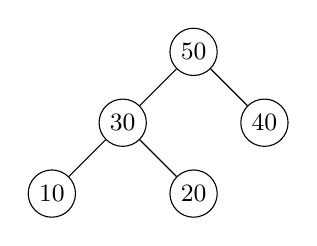
\begin{tikzpicture}[level distance=9mm, sibling distance=18mm,
    every node/.style={circle, draw, minimum size=6mm, inner sep=0pt, font=\small}]
    \node {50}
        child {node {30} child {node {10}} child {node {20}}}
        child {node {40}};
\end{tikzpicture}
\end{center}

Step 1: attach $42$ as right child of $40$ (first empty slot):

\begin{center}
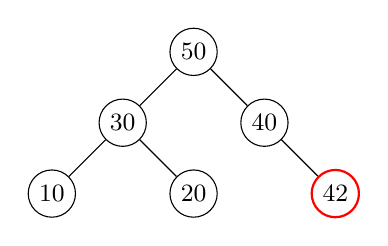
\begin{tikzpicture}[level distance=9mm, sibling distance=18mm,
    every node/.style={circle, draw, minimum size=6mm, inner sep=0pt, font=\small}]
    \node {50}
        child {node {30} child {node {10}} child {node {20}}}
        child {node {40} child[missing] {} child {node[draw=red, thick] {42}}};
\end{tikzpicture}
\end{center}

Step 2: $42 > 40$? Yes. Swap.

\begin{center}
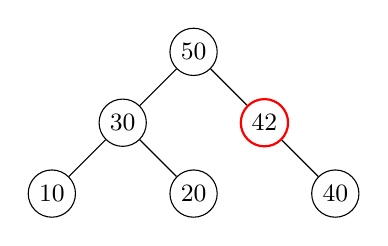
\begin{tikzpicture}[level distance=9mm, sibling distance=18mm,
    every node/.style={circle, draw, minimum size=6mm, inner sep=0pt, font=\small}]
    \node {50}
        child {node {30} child {node {10}} child {node {20}}}
        child {node[draw=red, thick] {42} child[missing] {} child {node {40}}};
\end{tikzpicture}
\end{center}

Step 3: $42 > 50$? No. Stop. Heap property restored.

\subsection*{Remove (max): replace-and-percolate-down}

\begin{enumerate}[leftmargin=*]
    \item Save the root's value (that's the answer we return).
    \item Take the \emph{last} node (rightmost leaf of the deepest level) and put it at the root. Delete the now-duplicate last slot. This preserves completeness but usually breaks the heap property at the root.
    \item Percolate down: compare the new root against its two children. If the larger child is greater than the node, swap with that child. Repeat until no larger child exists or the node reaches a leaf.
\end{enumerate}

The ``replace with last then percolate down'' dance is the whole algorithm. You're not finding a replacement by careful search -- you grab the structural last node to keep the tree complete, and then let percolate-down sort out the resulting local violation.

\begin{ideabox}
Heaps are the cleanest example in this course of \emph{trading generality for speed}. They give up ordered search, in-order traversal, and range queries -- capabilities a BST provides -- to get a guaranteed $O(1)$ peek and $O(\log n)$ insert/extract with a tiny implementation. Whenever you only need the extremum (and not ordered iteration), reach for a heap first.
\end{ideabox}

\subsection*{In the C++ STL}

\texttt{std::priority\_queue} is a max-heap by default, built on top of \texttt{std::vector}:

\begin{lstlisting}
#include <queue>
std::priority_queue<int> pq;        // max-heap of ints
pq.push(30); pq.push(50); pq.push(40);
std::cout << pq.top();              // 50
pq.pop();
std::cout << pq.top();              // 40
\end{lstlisting}

For a min-heap, pass \texttt{std::greater}:

\begin{lstlisting}
std::priority_queue<int, std::vector<int>, std::greater<int>> minpq;
\end{lstlisting}

Section 7.2 will show how the tree is actually stored -- surprise, not with pointers. Sections 7.3 and 7.4 formalize \texttt{percolateUp} and \texttt{percolateDown}. Section 7.5 builds the priority-queue ADT on top.

\section{7.2 Heaps Stored in Arrays}

Here's the twist: the binary tree in chapter 6 uses a \texttt{TreeNode} struct with \texttt{left}, \texttt{right}, (\texttt{parent}) pointers per node. A heap uses \textbf{nothing of the sort.} A heap is almost always stored as a plain array, with all parent/child relationships computed by \emph{index arithmetic}. No pointers, no allocations per node, no cache misses on node traversal. This is the single biggest reason the heap is the go-to priority queue in practice.

\begin{defnbox}[Array representation of a complete binary tree]
Number the nodes level by level, left to right, starting from the root at index 0. For a node at index $i$:
\[
\text{parent}(i) = \left\lfloor \frac{i-1}{2} \right\rfloor
\qquad
\text{leftChild}(i) = 2i + 1
\qquad
\text{rightChild}(i) = 2i + 2
\]
These formulas require the tree to be \emph{complete} -- every level full except possibly the last, which fills left-to-right. That's exactly the property heap operations preserve.
\end{defnbox}

\subsection*{Example}

\begin{center}
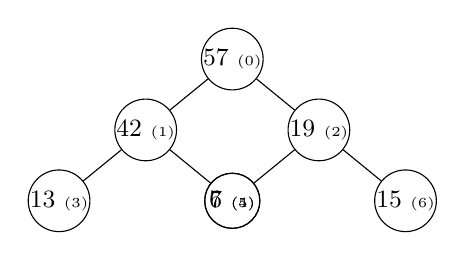
\begin{tikzpicture}[level distance=9mm, sibling distance=22mm,
    every node/.style={circle, draw, minimum size=7mm, inner sep=0pt, font=\small}]
    \node {57 \tiny(0)}
        child {node {42 \tiny(1)}
            child {node {13 \tiny(3)}}
            child {node {6 \tiny(4)}}
        }
        child {node {19 \tiny(2)}
            child {node {7 \tiny(5)}}
            child {node {15 \tiny(6)}}
        };
\end{tikzpicture}
\end{center}

stored as:
\begin{center}
\begin{tabular}{|c|c|c|c|c|c|c|c|}
\hline
Index & 0 & 1 & 2 & 3 & 4 & 5 & 6 \\
\hline
Value & 57 & 42 & 19 & 13 & 6 & 7 & 15 \\
\hline
\end{tabular}
\end{center}

Check: \texttt{parent(4) = (4-1)/2 = 1}, so parent of $6$ is $42$ -- correct. \texttt{leftChild(2) = 5}, so left child of $19$ is $7$ -- correct.

\begin{ideabox}
A \emph{complete} binary tree has no gaps, so every array slot corresponds to an actual node. That's why the index formulas work -- if the tree had missing internal nodes, you'd need sentinels or a different encoding. This is the crucial reason heap insert and remove are written to \emph{preserve completeness structurally first} and fix the heap-property violation second.
\end{ideabox}

\begin{examplebox}[Why the local property implies a global guarantee]
The max-heap property is stated \emph{locally}: each node is $\ge$ its
two children. The defnbox in \S7.1 claimed by transitivity that this
implies the \emph{global} fact ``the root's key is $\ge$ every
descendant's key.'' Here is the proof.

\textbf{Claim.} For every node $i$ and every descendant $j$ of $i$,
$\text{key}(i) \ge \text{key}(j)$.

\textbf{Proof by induction on $d = \text{depth}(j) - \text{depth}(i)$,
the depth difference between $j$ and $i$.}

\textit{Base case ($d = 1$)}. If $d = 1$, then $j$ is a child of $i$.
The local max-heap property at $i$ states $\text{key}(i) \ge
\text{key}(j)$ directly.

\textit{Inductive step ($d \ge 2$)}. Assume the claim holds for every
pair with depth difference $< d$. Let $j$ be a descendant of $i$ at
depth $d$ below $i$, and let $k$ be the parent of $j$. Then $k$ is a
descendant of $i$ at depth difference $d - 1$, so by the inductive
hypothesis $\text{key}(i) \ge \text{key}(k)$. The local max-heap
property at $k$ gives $\text{key}(k) \ge \text{key}(j)$. Chaining,
$\text{key}(i) \ge \text{key}(k) \ge \text{key}(j)$. \emph{Q.E.D.}

\textbf{Consequence.} Setting $i$ to the root: the root's key is $\ge$
every key in the heap, so \texttt{find\_max} is just ``return $h[0]$''
in $O(1)$. The minimum, by contrast, can be \emph{anywhere among the
leaves}, so \texttt{find\_min} on a max-heap is $\Omega(n)$ -- you have
to look at all of them. We will revisit this in \S7.6.
\end{examplebox}

\subsection*{Why arrays beat pointers here}

\begin{center}
\begin{tabular}{ll}
Pointer-based tree       & Array-based heap \\
\hline
3 pointers per node (24 B on 64-bit) & No per-element overhead \\
Cache miss per child jump           & Cache-friendly (children are 1--2 cells ahead) \\
\texttt{new}/\texttt{delete} per insert/remove & \texttt{vector} grows amortized $O(1)$ \\
Works for arbitrary tree shapes     & Requires completeness \\
\end{tabular}
\end{center}

For a heap of a million ints: pointer representation is $\approx 28$ MB of overhead beyond the values themselves; array representation is $\approx 0$ overhead. The array form is also a contiguous memory block, so sequential scans (like heapsort) are prefetch-friendly.

\subsection*{Percolate-up, array version}

Starting at some index \texttt{i} where the heap property might be broken upward, walk toward the root swapping with parent while the child is larger:

\begin{lstlisting}
void maxHeapPercolateUp(int i, std::vector<int>& h) {
    while (i > 0) {
        int parent = (i - 1) / 2;
        if (h[i] <= h[parent]) return;          // heap property satisfied
        std::swap(h[i], h[parent]);
        i = parent;                              // continue from new position
    }
}
\end{lstlisting}

The loop runs at most $\lfloor \log_2 n \rfloor$ times because each iteration halves the index. That's the $O(\log n)$ insert bound.

\subsection*{Percolate-down, array version}

Starting at some index \texttt{i} (usually 0, after the root was replaced), walk toward the leaves swapping with the larger child while a child is larger than the node:

\begin{lstlisting}
void maxHeapPercolateDown(int i, std::vector<int>& h) {
    int n = static_cast<int>(h.size());
    while (2 * i + 1 < n) {                      // at least one child exists
        int left  = 2 * i + 1;
        int right = 2 * i + 2;
        int biggest = left;
        if (right < n && h[right] > h[left]) biggest = right;
        if (h[i] >= h[biggest]) return;          // heap property satisfied
        std::swap(h[i], h[biggest]);
        i = biggest;
    }
}
\end{lstlisting}

Watch the three subtleties:
\begin{itemize}[leftmargin=*]
    \item \textbf{Check left first.} If \texttt{2*i+1 >= n}, \texttt{i} is a leaf and we're done.
    \item \textbf{Right might not exist.} That's why the right comparison is guarded by \texttt{right < n}.
    \item \textbf{Swap with the \emph{larger} child, not an arbitrary child.} If you swap with the smaller, the larger child becomes the new root and you've created a new violation below.
\end{itemize}

The loop runs at most $\lfloor \log_2 n \rfloor$ times (each iteration doubles the index). That's the $O(\log n)$ extract-max bound.

\begin{warnbox}
Off-by-one bugs are the dominant failure mode here. Triple-check your index formulas -- $(i-1)/2$ for parent uses integer division, which works because the formula is exact for both left ($i = 2p+1$) and right ($i = 2p+2$) children. Writing $i/2 - 1$ or $i/2$ will pass for some inputs and silently corrupt for others.
\end{warnbox}

\subsection*{Insert and extract, array versions}

\begin{lstlisting}
void maxHeapInsert(std::vector<int>& h, int value) {
    h.push_back(value);                          // step 1: preserve completeness
    maxHeapPercolateUp(h.size() - 1, h);         // step 2: restore heap property
}

int maxHeapExtract(std::vector<int>& h) {
    int top = h[0];
    h[0] = h.back();                             // move last to root
    h.pop_back();                                // shrink
    if (!h.empty()) maxHeapPercolateDown(0, h);
    return top;
}
\end{lstlisting}

Two functions, each $O(\log n)$ worst case, each three lines of logic. No tree allocations, no node structs, no parent pointers. The index formulas are the whole trick.

\begin{notebox}
\textbf{Zero-indexed vs.\ one-indexed.} Some textbooks and papers use index 1 as the root and leave index 0 unused. Then $\text{parent}(i) = i/2$, $\text{left}(i) = 2i$, $\text{right}(i) = 2i + 1$ -- slightly cleaner math. C++ code defaults to zero-indexed because \texttt{std::vector} is zero-indexed. Don't mix conventions in one codebase; pick one and stick with it. This course uses zero-indexed.
\end{notebox}

\section{7.3 Heapsort}

Heapsort is the sorting algorithm you get almost for free once you have a heap. The idea: turn an array into a max-heap, then repeatedly extract the max to the end of the array. You end up with an array sorted in ascending order, using \emph{no extra memory beyond the input array itself}.

Two phases:
\begin{enumerate}[leftmargin=*]
    \item \textbf{Heapify} the input array in place -- transform it into a valid max-heap.
    \item \textbf{Sort down}: swap \texttt{arr[0]} (the max) with the last unsorted slot, shrink the heap by one, and percolate the new root down. Repeat until the heap is empty.
\end{enumerate}

Both phases use one primitive: \texttt{maxHeapPercolateDown} from section 7.2.

\subsection*{Heapify: bottom-up heap construction}

Given an arbitrary array, how do we make it a max-heap? Naive approach: insert all elements one by one, each an $O(\log n)$ operation -- total $O(n \log n)$. There is a better way.

\begin{defnbox}[Heapify]
Call \texttt{percolateDown} on every internal node in reverse index order, from the last internal node down to the root. Leaves are trivially heaps (no children to violate anything), and each percolate-down restores the heap property over its subtree assuming the children are already valid heaps.
\end{defnbox}

The last internal node is at index $\lfloor n/2 \rfloor - 1$, because nodes at index $\ge \lfloor n/2 \rfloor$ are leaves (their first child index $2i + 1$ is out of range).

\begin{lstlisting}
void heapify(std::vector<int>& a) {
    for (int i = static_cast<int>(a.size()) / 2 - 1; i >= 0; --i)
        maxHeapPercolateDown(i, a);
}
\end{lstlisting}

\begin{examplebox}[Bottom-up build-max-heap on \texttt{[7,3,5,6,2,0,3,1,9,4]}]
$n = 10$, so the last internal node is at index $\lfloor 10/2 \rfloor -
1 = 4$. We call \texttt{percolateDown(i)} for $i = 4, 3, 2, 1, 0$ in
turn. At each step, the subtree rooted at the index being processed
becomes a valid max-heap; everything below it is already a valid
max-heap from prior steps.

\begin{center}
\begin{tabular}{|c|cccccccccc|l|}
\hline
Step & 0 & 1 & 2 & 3 & 4 & 5 & 6 & 7 & 8 & 9 & Action \\
\hline
start         & 7 & 3 & 5 & 6 & 2 & 0 & 3 & 1 & 9 & 4 & input array \\
$i=4$         & 7 & 3 & 5 & 6 & \textbf{4} & 0 & 3 & 1 & 9 & \textbf{2} & swap $a[4]=2$ with larger child $a[9]=4$ \\
$i=3$         & 7 & 3 & 5 & \textbf{9} & 4 & 0 & 3 & 1 & \textbf{6} & 2 & swap $a[3]=6$ with larger child $a[8]=9$ \\
$i=2$         & 7 & 3 & 5 & 9 & 4 & 0 & 3 & 1 & 6 & 2 & $a[2]=5 \ge \max(0,3)$, no swap \\
$i=1$         & 7 & \textbf{9} & 5 & \textbf{6} & 4 & 0 & 3 & 1 & \textbf{3} & 2 & swap $a[1]=3$ with $a[3]=9$, then $a[3]=3$ with $a[8]=6$ \\
$i=0$ swap 1  & \textbf{9} & \textbf{7} & 5 & 6 & 4 & 0 & 3 & 1 & 3 & 2 & swap $a[0]=7$ with $a[1]=9$ \\
$i=0$ swap 2  & 9 & \textbf{7} & 5 & \textbf{6} & 4 & 0 & 3 & 1 & 3 & 2 & at index 1, $a[1]=7 \ge \max(6,4)$, stop \\
\hline
\end{tabular}
\end{center}

Final: \texttt{[9, 7, 5, 6, 4, 0, 3, 1, 3, 2]}. Spot-check: $9 \ge
\{7, 5\}$, $7 \ge \{6, 4\}$, $5 \ge \{0, 3\}$, $6 \ge \{1, 3\}$, $4
\ge \{2\}$. Valid max-heap. Total work: 5 calls to
\texttt{percolateDown} doing 1, 1, 0, 2, 1 swaps respectively -- 5
swaps total for $n = 10$, well under the worst-case $n \log_2 n
\approx 33$ that a one-by-one insert sequence would do.
\end{examplebox}

\subsection*{Why heapify is $O(n)$, not $O(n \log n)$}

This is the cleverness of bottom-up construction, and it catches most students off-guard on exams.

Percolate-down at index $i$ does work proportional to the \emph{height of the subtree rooted at $i$}, not the total height of the tree. A leaf has height 0 (does no work). A parent of leaves has height 1 (at most 1 swap). The root has height $\log n$. Summed over all nodes:

\[
\sum_{i=0}^{\lfloor \log n \rfloor} (\text{nodes at height } i) \cdot i
= \sum_{i=0}^{\lfloor \log n \rfloor} \frac{n}{2^{i+1}} \cdot i
= O(n)
\]

The geometric series in $i/2^i$ converges to a constant. Half the nodes are leaves (do 0 work), a quarter do at most 1 swap, an eighth do at most 2 swaps, and so on. The totals balance out to $O(n)$.

\begin{ideabox}
This is the right mental image: bottom-up heapify cheats the worst case because \emph{most of the nodes are near the bottom where their percolate-down has nothing to do.} Repeated insertion is $O(n \log n)$ because it forces every element through a full height's worth of potential swaps. Same final data structure, different total cost. Prefer heapify over ``insert one by one'' whenever you have all the data up front.
\end{ideabox}

\subsection*{The sort-down phase}

After heapify, \texttt{a[0]} holds the maximum. The classic ``swap with last, shrink heap, percolate down'' trick used in \texttt{maxHeapExtract} (section 7.2) -- but we keep the extracted value in the array instead of returning it:

\begin{lstlisting}
void heapSort(std::vector<int>& a) {
    heapify(a);

    int n = static_cast<int>(a.size());
    for (int end = n - 1; end > 0; --end) {
        std::swap(a[0], a[end]);            // move current max to its final spot
        maxHeapPercolateDown(0, a, end);    // heap is now indices [0, end)
    }
}
\end{lstlisting}

Notice the overloaded \texttt{percolateDown} here takes an explicit \texttt{size} parameter -- after each swap, the last slot is ``sorted off'' and the heap shrinks. You're not physically removing elements; you're just treating the suffix as already-sorted.

\subsection*{Walk-through}

Sort \texttt{[11, 21, 12, 13, 19, 15]}.

Step 1 -- heapify, starting at index $\lfloor 6/2 \rfloor - 1 = 2$:

\begin{center}
\begin{tabular}{lllllll}
Before: & 11 & 21 & 12 & 13 & 19 & 15 \\
percolateDown(2): node 12 vs children (15) -- swap 12, 15 \\
 & 11 & 21 & \textbf{15} & 13 & 19 & \textbf{12} \\
percolateDown(1): node 21 vs children (13, 19) -- already biggest \\
 & 11 & 21 & 15 & 13 & 19 & 12 \\
percolateDown(0): node 11 vs (21, 15) -- swap with 21; then 11 vs (13, 19) -- swap with 19 \\
 & \textbf{21} & \textbf{19} & 15 & 13 & \textbf{11} & 12 \\
\end{tabular}
\end{center}

Step 2 -- sort down:

\begin{center}
\begin{tabular}{llllllll}
 & 21 & 19 & 15 & 13 & 11 & 12 \\
swap a[0]=21, a[5]=12; heap size 5; percolate 12 $\to$ children (19, 15) swap 12,19; then (13,11) stay \\
 & 19 & 13 & 15 & 12 & 11 & \textbf{21} \\
swap a[0]=19, a[4]=11; size 4; percolate 11 $\to$ (13, 15) swap 11, 15; then (12) stay \\
 & 15 & 13 & 11 & 12 & \textbf{19} & 21 \\
swap a[0]=15, a[3]=12; size 3; percolate 12 $\to$ (13, 11) swap 12, 13 \\
 & 13 & 12 & 11 & \textbf{15} & 19 & 21 \\
swap a[0]=13, a[2]=11; size 2; percolate 11 $\to$ (12) swap \\
 & 12 & 11 & \textbf{13} & 15 & 19 & 21 \\
swap a[0]=12, a[1]=11; size 1; done \\
 & 11 & \textbf{12} & 13 & 15 & 19 & 21 \\
\end{tabular}
\end{center}

Final: \texttt{[11, 12, 13, 15, 19, 21]}. Sorted ascending.

\begin{examplebox}[Heap sort on \texttt{[7,3,5,6,2,0,3,1,9,4]}: the sort-down phase]
We finished the build-heap example for this array above with
\texttt{[9, 7, 5, 6, 4, 0, 3, 1, 3, 2]}. Now run the sort-down loop.
At each step we swap $a[0]$ with $a[\text{end}]$, decrement
\texttt{end} (the heap shrinks; the swapped-in max is now in its
final sorted position), and percolate the new root down within the
prefix $a[0 \ldots \text{end}-1]$.

\begin{center}
\renewcommand{\arraystretch}{1.05}
\begin{tabular}{|c|cccccccccc|l|}
\hline
end & 0 & 1 & 2 & 3 & 4 & 5 & 6 & 7 & 8 & 9 & note \\
\hline
9 & 9 & 7 & 5 & 6 & 4 & 0 & 3 & 1 & 3 & 2 & post-heapify \\
9 & 2 & 7 & 5 & 6 & 4 & 0 & 3 & 1 & 3 & \textbf{9} & swap $a[0] \leftrightarrow a[9]$ \\
9 & 7 & 6 & 5 & 3 & 4 & 0 & 3 & 1 & 2 & \textbf{9} & percolate down at 0 (heap = $a[0..8]$) \\
8 & 2 & 6 & 5 & 3 & 4 & 0 & 3 & 1 & \textbf{7} & 9 & swap $a[0] \leftrightarrow a[8]$ \\
8 & 6 & 4 & 5 & 3 & 2 & 0 & 3 & 1 & \textbf{7} & 9 & percolate down (heap = $a[0..7]$) \\
7 & 1 & 4 & 5 & 3 & 2 & 0 & 3 & \textbf{6} & 7 & 9 & swap $a[0] \leftrightarrow a[7]$ \\
7 & 5 & 4 & 3 & 3 & 2 & 0 & 1 & \textbf{6} & 7 & 9 & percolate down (heap = $a[0..6]$) \\
6 & 1 & 4 & 3 & 3 & 2 & 0 & \textbf{5} & 6 & 7 & 9 & swap $a[0] \leftrightarrow a[6]$ \\
6 & 4 & 3 & 3 & 1 & 2 & 0 & \textbf{5} & 6 & 7 & 9 & percolate down (heap = $a[0..5]$) \\
5 & 0 & 3 & 3 & 1 & 2 & \textbf{4} & 5 & 6 & 7 & 9 & swap $a[0] \leftrightarrow a[5]$ \\
5 & 3 & 2 & 3 & 1 & 0 & \textbf{4} & 5 & 6 & 7 & 9 & percolate down (heap = $a[0..4]$) \\
4 & 0 & 2 & 3 & 1 & \textbf{3} & 4 & 5 & 6 & 7 & 9 & swap $a[0] \leftrightarrow a[4]$ \\
4 & 3 & 2 & 0 & 1 & \textbf{3} & 4 & 5 & 6 & 7 & 9 & percolate down (heap = $a[0..3]$) \\
3 & 1 & 2 & 0 & \textbf{3} & 3 & 4 & 5 & 6 & 7 & 9 & swap $a[0] \leftrightarrow a[3]$ \\
3 & 2 & 1 & 0 & \textbf{3} & 3 & 4 & 5 & 6 & 7 & 9 & percolate down (heap = $a[0..2]$) \\
2 & 0 & 1 & \textbf{2} & 3 & 3 & 4 & 5 & 6 & 7 & 9 & swap $a[0] \leftrightarrow a[2]$ \\
2 & 1 & 0 & \textbf{2} & 3 & 3 & 4 & 5 & 6 & 7 & 9 & percolate down (heap = $a[0..1]$) \\
1 & 0 & \textbf{1} & 2 & 3 & 3 & 4 & 5 & 6 & 7 & 9 & swap $a[0] \leftrightarrow a[1]$, done \\
\hline
\end{tabular}
\end{center}

Final: \texttt{[0, 1, 2, 3, 3, 4, 5, 6, 7, 9]}. Sorted, in-place, no
auxiliary buffer used at any point. Each \texttt{percolateDown} on a
heap of size $k$ does at most $\log_2 k$ comparisons; total cost is
$\sum_{k=1}^{n-1} \log_2 k = \Theta(n \log n)$, matching the bound.
\end{examplebox}

\subsection*{Cost analysis}

\begin{center}
\begin{tabular}{lll}
Phase & Per step & Total \\
\hline
Heapify              & up to $O(\log n)$ per node & $O(n)$ total (the geometric sum) \\
Sort-down            & $O(\log n)$ per extraction & $O(n \log n)$ \\
\hline
\textbf{Heapsort}    & & $\mathbf{O(n \log n)}$ \\
\end{tabular}
\end{center}

Space: $O(1)$ auxiliary. Heapsort is the canonical \emph{in-place} $O(n \log n)$ sort -- it rearranges the input array without needing a second array.

\subsection*{Heapsort vs.\ quicksort vs.\ mergesort}

\begin{center}
\begin{tabular}{llll}
Algorithm & Worst case & Space & Stable? \\
\hline
Quicksort   & $O(n^2)$      & $O(\log n)$ stack & no \\
Mergesort   & $O(n \log n)$ & $O(n)$            & yes \\
Heapsort    & $O(n \log n)$ & $O(1)$            & no \\
\end{tabular}
\end{center}

Heapsort's killer feature is the combination of $O(n \log n)$ \emph{worst case} and $O(1)$ auxiliary space. Quicksort has a worst case of $O(n^2)$; mergesort needs $O(n)$ extra memory. In practice, quicksort is usually fastest due to cache effects, but heapsort is picked when you need worst-case guarantees (embedded systems, real-time deadlines, adversarial inputs).

\begin{warnbox}
Heapsort is \textbf{not stable}: equal keys may swap order during the percolate steps. If stability matters (sorting records by one field without disturbing existing order on another), use mergesort or a stable quicksort variant, not heapsort.
\end{warnbox}

\begin{notebox}
\texttt{std::sort\_heap} and \texttt{std::make\_heap} in \texttt{<algorithm>} give you the two phases of heapsort. \texttt{std::partial\_sort} uses a heap-based algorithm to find and sort the top $k$ in $O(n \log k)$. None of these are the full \texttt{std::sort}, which typically uses introsort (quicksort that falls back to heapsort when recursion depth gets bad) -- precisely because heapsort's worst-case guarantee is the backup plan when quicksort starts to degrade.
\end{notebox}

\subsection*{Heap sort as priority-queue sort: the unifying table}

Recall the \S7.1 framing: every comparison sort is ``\texttt{build} a
priority queue, then $n$ \texttt{delete\_max}es.'' Different
implementations give different sorts:

\begin{center}
\begin{tabular}{lllll|l}
PQ implementation & \texttt{build} & \texttt{insert} & \texttt{delete\_max} & total ($n$ inserts + $n$ deletes) & in-place? \\
\hline
unsorted array          & $O(n)$ & $O(1)$       & $O(n)$       & $O(n^2)$  -- \textbf{selection sort} & yes \\
sorted array            & $O(n \log n)$ & $O(n)$       & $O(1)$       & $O(n^2)$  -- \textbf{insertion sort} & yes \\
balanced BST + max-ptr  & $O(n \log n)$ & $O(\log n)$  & $O(\log n)$  & $O(n \log n)$ -- \textbf{AVL sort} & no \\
\textbf{binary heap}    & $\mathbf{O(n)}$ & $\mathbf{O(\log n)}$ & $\mathbf{O(\log n)}$ & $\mathbf{O(n \log n)}$ -- \textbf{heap sort} & \textbf{yes} \\
\end{tabular}
\end{center}

The bottom row is the goal -- the only PQ here that hits $O(n \log n)$
total \emph{and} runs in-place. AVL sort matches heap sort's
asymptotics but needs $O(n)$ auxiliary space for the tree nodes plus
their pointers; selection and insertion sort run in-place but at
$O(n^2)$. The binary heap is the structure that satisfies all three
constraints simultaneously, which is why it is the canonical PQ
implementation.

\begin{notebox}[The in-place heap-sort prefix trick]
The \texttt{heapSort} loop above is in-place because the heap and the
``already-sorted output'' share the same array. Conceptually we keep a
counter $|Q|$ for ``how many array slots currently belong to the
heap.''

\begin{itemize}[leftmargin=*]
    \item Initially $|Q| = n$ (whole array is the unordered input we
          will heapify).
    \item After heapify, $a[0 \ldots |Q|-1]$ is the heap; nothing is
          sorted yet.
    \item Each sort-down step: \texttt{swap(a[0], a[|Q|-1])} sends the
          current max to position $|Q|-1$, then $|Q| \mathrel{-}= 1$
          shrinks the heap. The slot just vacated is now part of the
          \emph{sorted suffix} and is invisible to subsequent
          \texttt{percolateDown} calls (that's what passing
          \texttt{end} as the array bound enforces).
    \item Termination: when $|Q| = 1$, the suffix $a[1 \ldots n-1]$ is
          sorted and $a[0]$ holds the smallest, so the entire array is
          sorted.
\end{itemize}

The same array slot serves two roles at different points in the
algorithm -- ``part of the heap'' early, ``part of the sorted suffix''
late. That is the entire reason heap sort can be written without an
auxiliary buffer; merge sort cannot do this because its merge step
\emph{simultaneously} reads from two ranges and writes to a third.
\end{notebox}

\begin{notebox}[Sequence AVL Tree as a PQ alternative]
The PQ-sort table above lists ``balanced BST $+$ max-ptr'' as a row
with the same asymptotic bounds as the binary heap. That row is real:
augment a balanced BST (chapter 9: AVL or red-black) so that every
node carries a pointer (or index) to the maximum-key node in its
subtree. Maintenance is $O(1)$ extra work per rotation and per
insert/delete -- the augmentation propagates by ``my max is the
biggest of \{my key, my left subtree's max, my right subtree's
max\}.''

With that augmentation:
\begin{itemize}[leftmargin=*]
    \item \texttt{find\_max} = follow the root's max-pointer:
          $O(1)$.
    \item \texttt{insert} = standard BST insert + AVL rebalance,
          fixing up max-pointers along the path: $O(\log n)$.
    \item \texttt{delete\_max} = follow max-pointer, splice that
          node, fix-up: $O(\log n)$.
    \item \texttt{build} from $n$ items: $O(n \log n)$ (no analogue
          of bottom-up heapify's geometric trick).
\end{itemize}

Same $O(\log n)$ bounds as the binary heap on the steady-state ops.
Why not use it instead? Two reasons. (1) The AVL implementation is
roughly $10\times$ the code of a heap (chapter 9 makes that
concrete). (2) AVL sort cannot run in-place; the tree needs $O(n)$
nodes worth of pointer storage.

The AVL-as-PQ structure does become useful when you also need
\emph{ordered iteration} (chapter 9's bread and butter) on top of the
PQ ops -- something a heap cannot do efficiently. For the pure PQ
job, the heap wins on simplicity and locality.
\end{notebox}

\section{7.4 The Priority Queue ADT}

Section 7.1 motivated heaps with the priority-queue use case. This section formalizes the \emph{abstract data type} (ADT) and shows why heaps are the near-universal implementation. An ADT is a specification of operations and their contracts -- it tells you \emph{what} a data structure does, not \emph{how} it's implemented.

\begin{defnbox}[Priority queue]
A \textbf{priority queue} (PQ) is a collection where each element has a priority. The defining operations:
\begin{itemize}[leftmargin=*]
    \item \texttt{push(item)} -- insert an element.
    \item \texttt{pop()} -- remove and return the highest-priority element.
    \item \texttt{peek()} -- return (but don't remove) the highest-priority element.
    \item \texttt{isEmpty()} / \texttt{size()} -- the obvious.
\end{itemize}
``Highest priority'' can mean max-key or min-key depending on whether you want a max-PQ or min-PQ.
\end{defnbox}

Notice what the ADT \emph{doesn't} promise: arbitrary search, ordered iteration, range queries, positional access. A priority queue is FIFO ordered only among items of equal priority (that's the ``queue'' part), and even that is often not guaranteed unless the implementation makes a point of preserving it.

\subsection*{Two conventions for ``priority''}

A priority queue implementation has to answer: does the caller supply a priority alongside each item, or does the item carry its own priority?

\textbf{Separate-priority API:}

\begin{lstlisting}
pq.pushWithPriority(jobPointer, priorityNumber);
auto best = pq.pop();   // returns the stored item (not the priority)
\end{lstlisting}

Natural when the same object might live in multiple PQs with different priorities (e.g., a process could be in a CPU scheduler keyed by niceness and in an I/O scheduler keyed by deadline).

\textbf{Self-priority API:}

\begin{lstlisting}
struct Customer { std::string name; int waitScore; };
// ordering comparator compares on waitScore
pq.push(customer);
auto next = pq.pop();
\end{lstlisting}

Natural when priority is a property of the item itself. This is what \texttt{std::priority\_queue} does -- it takes a comparator and compares items directly.

Both are just different ways to express the same underlying concept. The self-priority API typically requires a comparator; the separate-priority API stores \texttt{(priority, item)} pairs and compares on the first component.

\subsection*{Contract summary}

\begin{center}
\begin{tabular}{lll}
Operation & Pre-condition & Post-condition \\
\hline
\texttt{push(x)}     & heap has room (or is resizable) & $x$ is in the PQ; size $+1$ \\
\texttt{pop()}       & PQ is non-empty & returns the max/min; that item is removed; size $-1$ \\
\texttt{peek()}      & PQ is non-empty & returns the max/min; PQ unchanged \\
\texttt{isEmpty()}   & none & true iff size $= 0$ \\
\texttt{size()}      & none & returns non-negative count \\
\end{tabular}
\end{center}

Violating the pre-condition (\texttt{pop} on empty) is undefined behavior in C++'s \texttt{std::priority\_queue}; Java's \texttt{PriorityQueue} returns null or throws \texttt{NoSuchElementException} depending on which method you call (\texttt{poll} vs.\ \texttt{remove}). Always check \texttt{isEmpty()} first, or wrap the call in a try/check.

\subsection*{Why heaps are the default implementation}

\begin{center}
\begin{tabular}{lllll}
Backing structure & push & pop (max) & peek & extra notes \\
\hline
Unsorted array/list   & $O(1)$      & $O(n)$     & $O(n)$ & peek rescans \\
Sorted array          & $O(n)$      & $O(1)$     & $O(1)$ & insert shifts \\
Sorted linked list    & $O(n)$      & $O(1)$     & $O(1)$ & insert scans \\
Balanced BST          & $O(\log n)$ & $O(\log n)$ & $O(\log n)$ & overkill, higher constants \\
\textbf{Binary heap}  & $O(\log n)$ & $O(\log n)$ & $O(1)$  & tight constants, cache-friendly \\
Fibonacci heap        & $O(1)$ amort. & $O(\log n)$ amort. & $O(1)$ & complex, big constants \\
\end{tabular}
\end{center}

The binary heap is the \emph{simplest} structure that gives log-factor bounds on both push and pop with $O(1)$ peek. It's also the one where the implementation is small, cache-friendly, and easy to reason about. Fibonacci heaps have better asymptotic bounds but their constant factors are so bad they're only a win at sizes real problems don't usually reach.

\subsection*{Mapping PQ operations to heap operations}

\begin{center}
\begin{tabular}{lll}
PQ op & Heap op (section 7.2) & Cost \\
\hline
\texttt{push(x)}   & \texttt{maxHeapInsert}: push to back, percolate up & $O(\log n)$ \\
\texttt{pop()}     & \texttt{maxHeapExtract}: swap root/last, pop, percolate down & $O(\log n)$ \\
\texttt{peek()}    & return \texttt{h[0]} & $O(1)$ \\
\texttt{isEmpty()} & return \texttt{h.empty()} & $O(1)$ \\
\texttt{size()}    & return \texttt{h.size()} & $O(1)$ \\
\end{tabular}
\end{center}

A priority queue is, in essentially all real codebases, just a thin wrapper around a heap's array.

\subsection*{Implementation sketch in C++}

\begin{lstlisting}
template <typename T, typename Cmp = std::less<T>>
class PriorityQueue {
    std::vector<T> h_;
    Cmp cmp_;   // cmp_(a, b) == true means "a has lower priority than b"
                // For a max-heap with std::less, cmp_(a, b) is a < b,
                // which is what we percolate up on.

    void percolateUp(std::size_t i) {
        while (i > 0) {
            std::size_t p = (i - 1) / 2;
            if (!cmp_(h_[p], h_[i])) return;        // parent is larger already
            std::swap(h_[p], h_[i]);
            i = p;
        }
    }
    void percolateDown(std::size_t i) {
        std::size_t n = h_.size();
        while (2 * i + 1 < n) {
            std::size_t l = 2 * i + 1, r = 2 * i + 2, best = l;
            if (r < n && cmp_(h_[l], h_[r])) best = r;
            if (!cmp_(h_[i], h_[best])) return;
            std::swap(h_[i], h_[best]);
            i = best;
        }
    }
public:
    bool empty() const { return h_.empty(); }
    std::size_t size() const { return h_.size(); }
    const T& peek() const { return h_.front(); }

    void push(T value) {
        h_.push_back(std::move(value));
        percolateUp(h_.size() - 1);
    }
    T pop() {
        T top = std::move(h_.front());
        h_.front() = std::move(h_.back());
        h_.pop_back();
        if (!h_.empty()) percolateDown(0);
        return top;
    }
};
\end{lstlisting}

That's 40 lines for a complete priority queue. The \texttt{std::priority\_queue} in the standard library is essentially this, with a few more template knobs.

\subsection*{Using \texttt{std::priority\_queue}}

\begin{lstlisting}
#include <queue>
#include <vector>

// Max-heap of ints
std::priority_queue<int> maxPQ;
maxPQ.push(5); maxPQ.push(1); maxPQ.push(9);
maxPQ.top();   // 9
maxPQ.pop();
maxPQ.top();   // 5

// Min-heap of ints
std::priority_queue<int, std::vector<int>, std::greater<int>> minPQ;

// Custom comparator on (priority, payload) pairs
using Entry = std::pair<int, std::string>;
auto cmp = [](const Entry& a, const Entry& b) { return a.first > b.first; };
std::priority_queue<Entry, std::vector<Entry>, decltype(cmp)> jobs(cmp);
jobs.push({3, "cleanup"}); jobs.push({1, "urgent"});
jobs.top();   // {1, "urgent"}   -- lower numeric priority = more urgent
\end{lstlisting}

\begin{warnbox}
\texttt{std::priority\_queue::top} returns a \emph{const reference}. You cannot mutate the top element in place -- attempting to \texttt{const\_cast} it and rewrite would break the heap invariant. If you need to change a priority, you have to \texttt{pop} the item and \texttt{push} a new one, or switch to a structure with an \texttt{increase\_key} / \texttt{decrease\_key} operation (indexed heap, \texttt{std::multiset}, or a hand-written heap with a side-index).
\end{warnbox}

\begin{ideabox}
An ADT separates ``what a structure promises'' from ``how it does it.'' Everywhere in this course, when a problem reduces to ``I keep needing the extremum of a changing set,'' you should reach for a priority queue -- and under the hood, you can bet it's a heap.
\end{ideabox}

\subsection*{\texttt{HEAP-INCREASE-KEY}: bumping a key upward}

The basic PQ interface only lets you \texttt{push} new items and
\texttt{pop} the extremum. Many real workloads need a fifth operation:
\textbf{change the priority of an item already in the queue}. The
canonical use case is \textbf{Dijkstra's algorithm} (chapter 10):
when a relaxation step finds a shorter path to a frontier vertex
$v$, we have to lower $v$'s key in the min-PQ. We don't want to pop
$v$ and re-push -- that's $O(n)$ to find $v$ in an unindexed heap.
We want a direct $O(\log n)$ operation that updates $v$'s key
\emph{in-place} and re-establishes the heap invariant.

For a max-heap, the operation is \textbf{increase-key} (the dual
\textbf{decrease-key} is the min-heap version). Algorithm:

\begin{enumerate}[leftmargin=*]
    \item Caller hands us the index $i$ of the slot to update and a
          new key $k$ that is \emph{not smaller} than the current
          key (otherwise the operation is undefined for a max-heap).
    \item Write $k$ into $h[i]$.
    \item \texttt{percolateUp(i)} -- the new key may now violate the
          heap property against its ancestors.
\end{enumerate}

Step 3 alone suffices because increasing a key cannot create a
violation \emph{below} $i$ -- $h[i]$'s descendants are still smaller
than the old (smaller) key, hence smaller than the new (larger)
key. The fix is one-directional and runs in $O(\log n)$.

\begin{lstlisting}
// Max-heap: raise h[i] to newKey (newKey must be >= current h[i]).
// Restores the heap property by percolating up from i.
void heapIncreaseKey(std::vector<int>& h, std::size_t i, int newKey) {
    if (newKey < h[i]) return;          // contract violation, no-op
    h[i] = newKey;
    while (i > 0) {
        std::size_t p = (i - 1) / 2;
        if (h[p] >= h[i]) return;
        std::swap(h[p], h[i]);
        i = p;
    }
}

// Min-heap mirror: lower h[i] to newKey (newKey must be <= current h[i]).
// This is what Dijkstra calls on every relaxation.
void heapDecreaseKey(std::vector<int>& h, std::size_t i, int newKey) {
    if (newKey > h[i]) return;
    h[i] = newKey;
    while (i > 0) {
        std::size_t p = (i - 1) / 2;
        if (h[p] <= h[i]) return;
        std::swap(h[p], h[i]);
        i = p;
    }
}
\end{lstlisting}

The operations \texttt{insert} and \texttt{increase-key} are sister
algorithms: \texttt{insert} is precisely ``append a sentinel
$-\infty$ at the end, then \texttt{increase-key} on that slot to the
real value.'' CLRS phrases \texttt{MAX-HEAP-INSERT} this way
explicitly.

\textbf{The catch.} \texttt{heapIncreaseKey} as written takes an
array index $i$. In a real workload the caller knows ``the vertex
$v$,'' not ``the array slot.'' You either maintain a side table
$\text{pos}[v] = i$ (updated by every \texttt{percolateUp} /
\texttt{percolateDown} swap) -- this is the \textbf{indexed heap} or
\textbf{indirect heap} -- or you use a structure that supports
search natively (\texttt{std::set}, hand-written balanced BST). The
indexed heap is the standard answer for Dijkstra implementations.

\begin{examplebox}[Insert and delete-max on a 7-element heap]
Start with the max-heap \texttt{[50, 30, 40, 10, 20, 35, 25]} (which
the array represents as the complete tree below).

\begin{center}
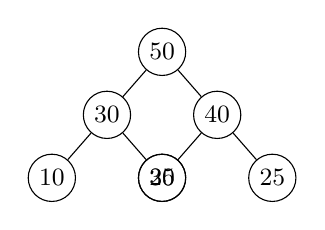
\begin{tikzpicture}[level distance=8mm, sibling distance=14mm,
    every node/.style={circle, draw, minimum size=6mm, inner sep=0pt, font=\small}]
    \node {50}
        child {node {30} child {node {10}} child {node {20}}}
        child {node {40} child {node {35}} child {node {25}}};
\end{tikzpicture}
\end{center}

\textbf{Insert 60.} Append at index 7 (next free slot, right child of
\texttt{30}): \texttt{[50, 30, 40, 10, 20, 35, 25, 60]}. Percolate up:
\begin{itemize}[leftmargin=*]
    \item $i=7$, parent $= 3$, $a[7]=60 > a[3]=10$, swap $\to$
          \texttt{[50, 30, 40, 60, 20, 35, 25, 10]}, $i=3$.
    \item $i=3$, parent $= 1$, $a[3]=60 > a[1]=30$, swap $\to$
          \texttt{[50, 60, 40, 30, 20, 35, 25, 10]}, $i=1$.
    \item $i=1$, parent $= 0$, $a[1]=60 > a[0]=50$, swap $\to$
          \texttt{[60, 50, 40, 30, 20, 35, 25, 10]}, $i=0$. Stop.
\end{itemize}

The percolate-up path was $7 \to 3 \to 1 \to 0$, three swaps -- exactly
the height of the tree. Heap property restored.

\textbf{Now \texttt{delete\_max} from the result.} Save $60$, move
last ($10$) to root, pop: \texttt{[10, 50, 40, 30, 20, 35, 25]}.
Percolate down:
\begin{itemize}[leftmargin=*]
    \item $i=0$: children are $a[1]=50$, $a[2]=40$. Larger child is
          $a[1]=50$; $a[0]=10 < 50$, swap $\to$
          \texttt{[50, 10, 40, 30, 20, 35, 25]}, $i=1$.
    \item $i=1$: children are $a[3]=30$, $a[4]=20$. Larger is
          $a[3]=30$; $a[1]=10 < 30$, swap $\to$
          \texttt{[50, 30, 40, 10, 20, 35, 25]}, $i=3$.
    \item $i=3$: children are $a[7]=$ out of range, so $i=3$ is a
          leaf. Stop.
\end{itemize}

The percolate-down path was $0 \to 1 \to 3$, again three swaps.
Returned value: $60$. Final array: \texttt{[50, 30, 40, 10, 20, 35,
25]} -- exactly what we started with, as expected (insert + delete
of the new max is a round-trip).
\end{examplebox}

\begin{notebox}[Set vs.\ Multiset on a heap]
A \emph{Set} treats keys as unique: inserting a key already present
either rejects the second copy or overwrites it. A \emph{Multiset}
allows duplicates -- a counter, a histogram, a stream of repeated
events.

Heaps natively implement the \textbf{Multiset} interface. Two
elements with the same key sit comfortably in the array side by
side; the heap property uses $\ge$ (not $>$), so equal-key parent
and child satisfy the local invariant. Repeated \texttt{insert} of
the same key just appends, and \texttt{delete\_max} pops them in
some unspecified order on ties.

If you need a true Set, layer one on top: keep a separate
\texttt{std::unordered\_set<key>} for membership tests and reject
duplicates at the PQ boundary. Or switch to an AVL/RB tree
(chapter 9), where the Set/Multiset distinction is a single template
parameter (\texttt{std::set} vs.\ \texttt{std::multiset}).
\end{notebox}

\section{7.5 Treaps: Heap + BST}

\textbf{This is your introduction to rotations.} We meet them in the
simplest setting (the treap), where their job is just ``percolate a
high-priority node upward without breaking BST order.'' Chapter 9
generalises the same primitive to AVL trees and red-black trees, where
rotations restore strict balance invariants instead of probabilistic
ones. The mechanics are identical across all three structures; only
the trigger -- ``what condition fires a rotation?'' -- changes. Master
the geometry here and chapter 9's case analysis will land cleanly.

Chapter 6 ended with a warning: a raw BST collapses on sorted input. Chapter 6.10 teased self-balancing trees (AVL, red-black) as the rigorous fix. This section shows a \emph{lazier} fix -- a fix that doesn't require tracking balance factors or recoloring -- called a \textbf{treap} (tree + heap).

\begin{defnbox}[Treap]
A treap is a binary tree where each node carries two keys:
\begin{itemize}[leftmargin=*]
    \item A \textbf{main key} (the data you care about), maintained in \emph{BST order} across the tree.
    \item A \textbf{priority} (a random number chosen when the node is inserted), maintained in \emph{heap order} across the tree.
\end{itemize}
Both invariants hold simultaneously: for every node $n$, main-keys follow the BST rule w.r.t.\ subtrees, and priorities follow the heap rule w.r.t.\ parent/child.
\end{defnbox}

The magic observation: \emph{given a set of (main key, priority) pairs with distinct priorities, there is exactly one tree shape that satisfies both invariants.} The highest-priority node has to be the root (heap), and among its descendants the BST ordering is determined. So if priorities are random, the tree's shape is the same tree you'd get by inserting the main keys in the \emph{random order of their priorities}. And we already know: random-order BST insertion gives expected $O(\log n)$ height.

The treap is a self-balancing BST that achieves expected $O(\log n)$ operations by \emph{randomizing its insertion order internally}, without the caller having to cooperate.

\subsection*{The missing primitive: rotations}

Percolate-up in a normal heap swaps parent and child. That breaks the BST ordering. Treaps need a swap-like operation that \emph{preserves BST ordering}. That operation is the \textbf{rotation}, the same move AVL and red-black trees use.

\begin{defnbox}[Right rotation]
If $y$ is a node with left child $x$, right-rotating at $y$ makes $x$ the new root of the subtree, $y$ becomes $x$'s right child, and $x$'s former right child $B$ becomes $y$'s new left child. Left rotation is the mirror image.
\end{defnbox}

\begin{center}
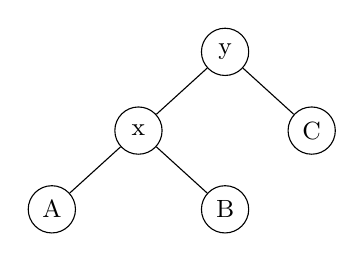
\begin{tikzpicture}[level distance=10mm, sibling distance=22mm,
    every node/.style={circle, draw, minimum size=6mm, inner sep=0pt, font=\small}]
    \node {y}
        child {node {x}
            child {node {A}}
            child {node {B}}
        }
        child {node {C}};
\end{tikzpicture}
\quad $\xrightarrow{\text{rotate right at } y}$ \quad
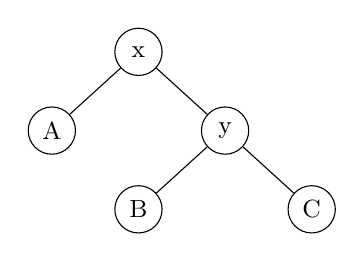
\begin{tikzpicture}[level distance=10mm, sibling distance=22mm,
    every node/.style={circle, draw, minimum size=6mm, inner sep=0pt, font=\small}]
    \node {x}
        child {node {A}}
        child {node {y}
            child {node {B}}
            child {node {C}}
        };
\end{tikzpicture}
\end{center}

Check ordering: before, $A < x < B < y < C$. After, still $A < x < B < y < C$. The in-order sequence is preserved. \emph{Heights and parent/child relationships change; BST ordering does not.}

Rotations are the universal self-balancing primitive. Once you have them, AVL, red-black, and treaps are all ``use rotations to restore some auxiliary invariant after a modification.'' The auxiliary invariant differs per structure; the mechanics are identical.

\subsection*{Treap insert}

\begin{enumerate}[leftmargin=*]
    \item Insert the new node at the right leaf position by main-key (pure BST insert).
    \item Assign it a random priority.
    \item While its priority exceeds its parent's priority, rotate so that the node moves up one level. \emph{Rotate right} if the node is a left child; \emph{rotate left} if it is a right child.
\end{enumerate}

The rotation choice is forced: to move a left-child upward, only a right-rotation at the parent works; analogously for a right-child and left-rotation. Each rotation preserves BST ordering and fixes one heap-property violation. After $O(\log n)$ expected rotations, the heap invariant is restored everywhere.

Example: start with a treap and insert key $B$ (assigned priority 70):

\begin{center}
\emph{After BST insert of B, before rotations:}
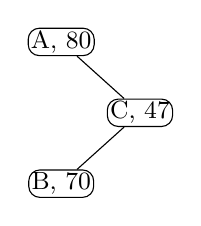
\begin{tikzpicture}[level distance=9mm, sibling distance=20mm,
    every node/.style={rectangle, draw, rounded corners, inner sep=1pt, font=\small}]
    \node {A, 80}
        child[missing] {}
        child {node {C, 47}
            child {node {B, 70}} child[missing] {}
        };
\end{tikzpicture}
\end{center}

Heap violation: parent \texttt{C}'s priority 47 is less than \texttt{B}'s 70. \texttt{B} is a left child, so rotate right at \texttt{C}:

\begin{center}
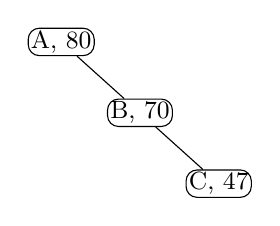
\begin{tikzpicture}[level distance=9mm, sibling distance=20mm,
    every node/.style={rectangle, draw, rounded corners, inner sep=1pt, font=\small}]
    \node {A, 80}
        child[missing] {}
        child {node {B, 70}
            child[missing] {}
            child {node {C, 47}}
        };
\end{tikzpicture}
\end{center}

Now \texttt{B}'s parent is \texttt{A} with priority 80 -- heap holds (80 $>$ 70). Stop. Treap restored.

\subsection*{Treap delete}

To delete a node $X$:
\begin{enumerate}[leftmargin=*]
    \item Pretend $X$'s priority is $-\infty$ (lowest possible). Now the heap property is violated at $X$: every child's priority is greater.
    \item Percolate $X$ down by rotating it with the \emph{higher-priority} child. That child becomes the new subtree root, $X$ sinks one level. Continue until $X$ has no children.
    \item Unhook and delete $X$.
\end{enumerate}

The ``higher-priority child'' rule matters: rotating with the \emph{lower}-priority child would leave a new heap violation in place of the old one. Rotating with the higher-priority child lifts it up and fixes the violation at that level.

Example: delete node \texttt{F} from a tree where its children are \texttt{C} (priority 29) and \texttt{I} (priority 13). Assign \texttt{F}'s priority to $-\infty$. Higher-priority child is \texttt{C}, so rotate right at \texttt{F} (moving \texttt{C} up). Continue until \texttt{F} has no children, then delete.

\subsection*{Cost analysis}

All treap operations have \textbf{expected} cost $O(\log n)$, because the tree shape is (in expectation) the shape of a BST built from $n$ items inserted in random order -- expected height $O(\log n)$.

\begin{center}
\begin{tabular}{lll}
Operation & Expected & Worst-case \\
\hline
Search & $O(\log n)$ & $O(n)$ \\
Insert & $O(\log n)$ & $O(n)$ \\
Delete & $O(\log n)$ & $O(n)$ \\
\end{tabular}
\end{center}

The worst case is still $O(n)$ -- if your random-number generator has really bad luck, you could get a skewed tree. But the probability of this is exponentially small, so in practice treaps perform as well as AVL or red-black trees while being substantially simpler to implement.

\begin{ideabox}
A treap doesn't guarantee balance -- it \emph{randomizes} to make imbalance improbable. This is a common pattern in computer science: don't solve the hard version (guaranteed balance, as in AVL / red-black); randomize the input to dodge worst cases (as in quicksort, hash-function-seeded hash tables, skip lists, treaps). When randomization is acceptable, it's almost always easier to implement than the deterministic version.
\end{ideabox}

\subsection*{Treaps vs.\ AVL vs.\ red-black}

\begin{center}
\begin{tabular}{llll}
Structure & Balance guarantee & Implementation complexity & Used by \\
\hline
AVL         & strict $O(\log n)$           & medium   & older DB indexes \\
Red-black   & $O(\log n)$ (weaker balance) & high     & \texttt{std::map}, Linux kernel \\
Treap       & expected $O(\log n)$         & \textbf{low} & competitive programming, teaching \\
Skip list   & expected $O(\log n)$         & low       & Redis, LevelDB \\
\end{tabular}
\end{center}

Treaps are rarely the choice in production standard libraries (AVL and red-black trees' deterministic guarantees matter for adversarial workloads), but they're popular in competitive-programming circles for their tiny implementation. Roughly 30 lines of C++ gets you a working treap; a working red-black tree is 10$\times$ that.

\begin{notebox}
The trick of ``attach a random secondary key and let it drive structure'' is deeply generalizable. Skip lists use it for levels (each node has a random ``tower height''). Probabilistic data structures in databases (HyperLogLog, Count-Min sketches) use it for bucket assignments. Treaps are a clean, easy-to-visualize introduction to the technique.
\end{notebox}

\section{7.6 Heap Exercises and Pitfalls}

This section collects four exercises that sharpen the difference
between ``heap'' and ``ordered structure,'' and two pitfalls that
catch students implementing heaps for the first time. The k-proximate
sorting result at the end is the showcase application of heap sort
beyond ``just sort an array'' -- it is what convinces a working
engineer that the heap is a load-bearing tool, not a textbook
curiosity.

\subsection*{Pitfall 1: the minimum of a max-heap is $\Omega(n)$}

\begin{warnbox}[Heaps are not BSTs -- minimum search costs you a linear scan]
\textbf{Claim.} Finding the minimum element in a max-heap of $n$ keys
requires inspecting $\Omega(n)$ array slots in the worst case. There
is no $O(\log n)$ algorithm.

\textbf{Sketch.} The max-heap property forces the root to hold the
maximum, but says \emph{nothing} about where the minimum lives -- it
must be a leaf (any non-leaf has at least one child smaller than
itself, so internal nodes can't be the minimum), but it can be
\textbf{any} of the $\lceil n/2 \rceil$ leaves. Without knowing
which leaf, you have to inspect them all. Algorithmic lower bound:
$\Theta(n)$.

\textbf{Why this matters.} Students who came up through BSTs
sometimes assume ``a balanced tree gives me $O(\log n)$ for any
query.'' False for heaps. Heaps are \emph{one-sided}: $O(1)$ to the
extremum at the root, $\Omega(n)$ to anything else.

If you need cheap access to both extrema simultaneously, you want a
\textbf{double-ended priority queue} (min-max heap, interval heap, or
two synchronised heaps with cross-pointers) -- a strictly more complex
structure. Or use an AVL/RB tree (chapter 9): $O(\log n)$ to either
extremum, plus ordered iteration as a bonus.
\end{warnbox}

\subsection*{Pitfall 2: max-heap to min-heap conversion is $O(n)$}

\begin{examplebox}[Re-running build-heap with the flipped property]
\textbf{Problem.} You have a valid max-heap stored in an array $A$ of
length $n$. You realise you want a min-heap of the same elements.
\textbf{Cost?}

\textbf{Naive answer.} Pop $n$ times into a buffer ($O(n \log n)$),
re-insert one-by-one into a fresh min-heap ($O(n \log n)$). Total
$O(n \log n)$.

\textbf{Better answer.} Just re-run \texttt{build\_heap} on the same
array with the comparator flipped. The bottom-up heapify procedure
doesn't care that the input was previously a valid max-heap -- it
treats the array as an arbitrary input and produces a valid heap of
the chosen orientation in $O(n)$.

\begin{lstlisting}
// Convert a valid max-heap in-place to a valid min-heap.
// Bottom-up heapify with the comparator flipped: O(n).
void maxToMinHeap(std::vector<int>& a) {
    auto percolateDownMin = [&](int i) {
        int n = static_cast<int>(a.size());
        while (2 * i + 1 < n) {
            int l = 2 * i + 1, r = 2 * i + 2, smallest = l;
            if (r < n && a[r] < a[l]) smallest = r;
            if (a[i] <= a[smallest]) return;
            std::swap(a[i], a[smallest]);
            i = smallest;
        }
    };
    for (int i = static_cast<int>(a.size()) / 2 - 1; i >= 0; --i)
        percolateDownMin(i);
}
\end{lstlisting}

The lesson: \emph{heap structure isn't directional.} The same complete
binary tree (and its array representation) supports either heap
property; the ``which is on top'' choice is just a comparator flip.
\end{examplebox}

\subsection*{The showcase application: $k$-proximate sorting in $O(n \log k)$}

\textbf{Problem.} An input stream of $n$ keys is \emph{$k$-proximate}:
every key is at most $k$ positions away from where it would land in
the sorted output. Sort the stream using only $O(k)$ extra memory and
$O(n \log k)$ time -- both of which beat general $O(n \log n)$ when
$k \ll n$.

\textbf{Where this comes from.} A real example: a sensor network sends
timestamped readings to a server. Network jitter shuffles the
arrivals slightly, but no reading is more than $k = 10$ positions
out of place. A streaming database has the same problem: events
arrive nearly-sorted by timestamp, with bounded skew. Naive
$O(n \log n)$ sort works but burns $O(n)$ memory; the streaming
algorithm we develop here uses just $O(k)$.

\textbf{Algorithm (sliding-window min-heap).}

\begin{enumerate}[leftmargin=*]
    \item Read the first $k+1$ items into a min-heap. (Why $k+1$? The
          true minimum of the entire output must be one of these,
          because no item arrives more than $k$ positions late.)
    \item For each subsequent input position $i = k+1, k+2, \ldots,
          n-1$:
          \begin{enumerate}[leftmargin=*]
              \item \texttt{delete\_min} from the heap; that's the
                    next sorted output element.
              \item \texttt{insert} input position $i$ into the heap.
          \end{enumerate}
    \item After the input is exhausted, drain the heap with
          \texttt{delete\_min} until empty. Those are the last $k+1$
          sorted output elements.
\end{enumerate}

\textbf{Correctness.} Inductively, when we are about to emit the
$j$-th output element (1-indexed), every input position
$\ge j + k + 1$ holds a key $\ge$ the true $j$-th smallest (because
that key would have to travel more than $k$ positions to land
earlier). So the true $j$-th smallest must already be in the heap
of size $k+1$, and it is the heap's minimum. Emit it.

\textbf{Cost.} Heap size never exceeds $k+1$. Each
\texttt{insert} and \texttt{delete\_min} costs $O(\log k)$. Total:
$O(n \log k)$, with $O(k)$ auxiliary space. When $k = O(1)$ this is
linear; when $k = \Theta(n)$ this matches general heap sort. The
algorithm is strictly better than ``sort everything'' whenever the
input has bounded skew.

\textbf{C++ port (OCW r08 algorithm in idiomatic C++17).} The OCW
recitation gives this in Python; here is the C++ rendering using
\texttt{std::priority\_queue} configured as a min-heap.

\begin{lstlisting}
#include <queue>
#include <vector>
#include <functional>

// Sort a k-proximate input in O(n log k) time, O(k) extra memory.
// Returns the sorted output as a fresh vector.
std::vector<int> kProximateSort(const std::vector<int>& input,
                                std::size_t k) {
    std::priority_queue<int, std::vector<int>, std::greater<int>> minHeap;
    std::vector<int> out;
    out.reserve(input.size());

    // Phase 1: prime the heap with the first k+1 items (or fewer
    // if input is shorter than k+1).
    std::size_t primed = std::min(k + 1, input.size());
    for (std::size_t i = 0; i < primed; ++i) minHeap.push(input[i]);

    // Phase 2: for each remaining input, emit the heap-min and push
    // the new input. Heap stays at size <= k+1.
    for (std::size_t i = primed; i < input.size(); ++i) {
        out.push_back(minHeap.top());
        minHeap.pop();
        minHeap.push(input[i]);
    }

    // Phase 3: drain whatever remains in the heap.
    while (!minHeap.empty()) {
        out.push_back(minHeap.top());
        minHeap.pop();
    }
    return out;
}
\end{lstlisting}

\textbf{Walk-through.} Take \texttt{input = [3, 1, 2, 6, 4, 5, 9, 7,
8]} with $k = 2$. (Verify $k$-proximacy: in the sorted output
\texttt{[1, 2, 3, 4, 5, 6, 7, 8, 9]}, the input's $3$ at position $0$
should land at sorted position $2$ -- offset $2$, OK. The $1$ at
position $1$ should land at position $0$ -- offset $1$, OK. And so
on.)

\begin{center}
\begin{tabular}{|c|l|l|l|}
\hline
step & action & heap (min on top) & output \\
\hline
prime & push 3, 1, 2 & \{1, 2, 3\} & [] \\
$i=3$ & emit min 1, push 6 & \{2, 3, 6\} & [1] \\
$i=4$ & emit min 2, push 4 & \{3, 4, 6\} & [1, 2] \\
$i=5$ & emit min 3, push 5 & \{4, 5, 6\} & [1, 2, 3] \\
$i=6$ & emit min 4, push 9 & \{5, 6, 9\} & [1, 2, 3, 4] \\
$i=7$ & emit min 5, push 7 & \{6, 7, 9\} & [1, 2, 3, 4, 5] \\
$i=8$ & emit min 6, push 8 & \{7, 8, 9\} & [1, 2, 3, 4, 5, 6] \\
drain & emit 7              & \{8, 9\}     & [1, 2, 3, 4, 5, 6, 7] \\
drain & emit 8              & \{9\}        & [1, 2, 3, 4, 5, 6, 7, 8] \\
drain & emit 9              & \{\}         & [1, 2, 3, 4, 5, 6, 7, 8, 9] \\
\hline
\end{tabular}
\end{center}

Sorted. Heap never exceeded size $k + 1 = 3$ even though the input
had 9 elements. Memory budget honoured.

\begin{ideabox}[Why $k$-proximate sorting is the showcase]
The full sort took $O(n \log n)$ time with $O(n)$ memory in chapter
3's sense. Here we shaved memory to $O(k)$ and (when $k \ll n$) time
to $O(n \log k)$ -- both wins driven entirely by the priority-queue
ADT and the bottom-up heap structure. The same idea (bounded-window
heap) underlies streaming top-$k$ queries, online median estimation
(two-heap trick), and event-loop schedulers. Heaps are the substrate
under all of them.
\end{ideabox}

\subsection*{Two implementation pitfalls}

\begin{warnbox}[Off-by-one on \texttt{parent} / \texttt{left} / \texttt{right}]
The zero-indexed formulas $\text{parent}(i) = \lfloor (i-1)/2
\rfloor$, $\text{left}(i) = 2i + 1$, $\text{right}(i) = 2i + 2$ are
\emph{not} the same as the one-indexed formulas $\text{parent}(i)
= \lfloor i/2 \rfloor$, $\text{left}(i) = 2i$, $\text{right}(i) = 2i +
1$. Mixing them within a single implementation produces silent
corruption -- the percolate routine traverses the tree as if it had a
different shape than the array stores, and items end up in the wrong
slots without any out-of-bounds error to flag the bug.

A common subtle mistake: writing $\text{parent}(i) = i / 2 - 1$
``because the formulas usually cancel.'' For $i = 1$ this gives
$\text{parent}(1) = 0$ (correct). For $i = 2$ it gives
$\text{parent}(2) = 0$ (correct). For $i = 3$ it gives
$\text{parent}(3) = 0$ (\emph{wrong} -- should be $1$). Test the
formula on at least three small indices before trusting it.
\end{warnbox}

\begin{warnbox}[Bounding the recursion when child indices overflow]
Both \texttt{percolateDown} variants must guard \emph{both} child
indices against the array bound. A leaf is any node where
$2i + 1 \ge n$ -- it has zero children. A half-leaf (one left child,
no right) is $2i + 1 < n$ but $2i + 2 \ge n$. The right-child
comparison must be guarded by \texttt{right < n}.

A common bug pattern:
\begin{lstlisting}
// BUG: dereferences a[2*i+2] without checking the bound.
int biggest = a[2*i+1] > a[2*i+2] ? 2*i+1 : 2*i+2;
\end{lstlisting}
On a heap of even size $n$ this reads past the end of the array. In
debug builds with bounds-checking iterators it traps; in release
builds it silently returns garbage and \texttt{percolateDown} swaps
with random memory. Always check \texttt{right < n} before using the
right child's value.
\end{warnbox}

\section{7.7 \texorpdfstring{$d$}{d}-ary Heaps and Forward Refs to Fibonacci}

So far ``heap'' has meant ``binary heap'' -- every internal node has
at most two children. That choice was arbitrary. Generalising to
$d$ children per node gives the \textbf{$d$-ary heap}, a one-line
algorithmic change with a real practical payoff in graph algorithms.

\subsection*{The generalisation}

\begin{defnbox}[$d$-ary heap]
A complete $d$-ary tree stored in an array, where each node has up to
$d$ children. Index arithmetic for a node at index $i$:
\[
\text{parent}(i) = \left\lfloor \frac{i - 1}{d} \right\rfloor,
\qquad
\text{child}_j(i) = d \cdot i + j + 1
\quad \text{for } j = 0, 1, \ldots, d - 1.
\]
The max-heap property is unchanged: every node is $\ge$ all its (up
to $d$) children. \texttt{percolateUp} is unchanged. \texttt{percolateDown}
must scan all $d$ children to find the largest.
\end{defnbox}

The tree height drops from $\Theta(\log_2 n)$ to $\Theta(\log_d n)$.
That looks like a free win, but \texttt{percolateDown} now does $d$
comparisons per level instead of $2$:

\begin{center}
\begin{tabular}{lll}
operation         & binary heap     & $d$-ary heap                    \\
\hline
\texttt{insert} / \texttt{increase\_key} & $\Theta(\log_2 n)$ & $\Theta(\log_d n)$ \\
\texttt{delete\_max}    & $\Theta(\log_2 n)$ & $\Theta(d \cdot \log_d n)$ \\
\texttt{find\_max}      & $\Theta(1)$         & $\Theta(1)$                   \\
\texttt{build\_heap}    & $\Theta(n)$         & $\Theta(n)$                   \\
\end{tabular}
\end{center}

\subsection*{Why $d = 4$ is common in production Dijkstra}

\textbf{Dijkstra's algorithm} on a graph with $V$ vertices and $E$
edges does $O(V)$ \texttt{delete\_min}s and $O(E)$
\texttt{decrease\_key}s. Total cost with a binary min-heap:
$O((V + E) \log V)$. With a $d$-ary heap:
$O(V \cdot d \log_d V + E \log_d V) = O((V \cdot d + E) \log_d V)$.

Choose $d$ to minimise this. Setting $d \approx E/V$ (the average
degree) gives $O(E \log_{E/V} V)$, which on dense graphs is
asymptotically faster than the binary-heap version. Empirically,
$d = 4$ tends to be the sweet spot on real machines: it cuts the tree
height by a factor of $\log_2 4 = 2$ vs.\ binary, and the
4-comparison \texttt{percolateDown} fits inside one cache line of
\texttt{int}s. This is what production routing engines and graph
analytics frameworks tend to use.

\begin{notebox}[The Fibonacci-heap forward ref]
Going further down the asymptotic-optimisation rabbit hole leads to
the \textbf{Fibonacci heap} (CLRS chapter 19), which gets
\texttt{decrease\_key} down to $O(1)$ amortised and brings Dijkstra
to $O(E + V \log V)$. The constants, however, are bad enough that on
real hardware the $d$-ary heap with $d \in \{4, 8\}$ usually beats
the Fibonacci heap up to graph sizes of $10^7$ vertices or so.
Fibonacci heaps are theoretically beautiful and practically
specialised -- worth knowing they exist (so you don't reinvent them),
not worth implementing unless your profiling has already eliminated
every other bottleneck. The CS 300 default substrate for graph
algorithms in chapter 10 is the binary min-heap; the $d$-ary
generalisation is the production-grade upgrade.
\end{notebox}

\begin{ideabox}[The big picture: heaps and what comes next]
\textbf{Heaps are the first non-trivial Set-ADT implementation in
this course.} Chapter 1 gave you arrays and sorted arrays as Set
implementations -- correct, but with $O(n)$ insert/delete bottlenecks.
This chapter delivered the binary heap: $O(\log n)$ on both
\texttt{insert} and \texttt{delete\_max}, $O(1)$ on \texttt{find\_max},
$O(n)$ on \texttt{build}, all in-place, all on a contiguous array.
That's the priority-queue ADT, period.

\textbf{Heaps don't do everything.} They do not support arbitrary
\texttt{find}, ordered iteration, range queries, predecessor /
successor lookups, or efficient \texttt{find\_min} (in a max-heap).
For those, you need a structure that maintains \emph{global} key
order, not just a local extremum invariant.

\textbf{Looking ahead.}
\begin{itemize}[leftmargin=*]
    \item \textbf{Chapter 9 (AVL and red-black trees)} delivers the
          full Set-with-ordered-iteration ADT in $O(\log n)$ per
          op. The rotation primitive you met in \S7.5 is the
          machinery; chapter 9 generalises the trigger from
          ``priority is too small'' (treap) to ``balance factor is
          out of $\{-1, 0, +1\}$'' (AVL) or ``two reds in a row''
          (red-black).
    \item \textbf{Chapter 10 (graph algorithms)} consumes the
          priority queue from this chapter wholesale.
          \textbf{Dijkstra} and \textbf{Prim} are essentially
          ``$|V|$ \texttt{delete\_min}s and $|E|$
          \texttt{decrease\_key}s'' on top of a min-PQ. The
          \texttt{decrease\_key} operation in \S7.4 is the
          relaxation primitive there.
    \item \textbf{Chapter 13 (sorting and search)} places
          \textbf{heap sort} in the comparison-sort table alongside
          quicksort, mergesort, counting sort, and radix sort. Heap
          sort's role: the worst-case $O(n \log n)$ in-place sort
          you fall back to when quicksort's randomised guarantees
          aren't enough (introsort uses exactly this fallback).
\end{itemize}

The single sentence to take away: \emph{the priority queue is the
ADT every algorithm involving ``next-most-important item'' needs,
and the binary heap is its near-universal implementation -- simple,
in-place, cache-friendly, correct.}
\end{ideabox}

\end{document}
